\documentclass[UKenglish]{uiomasterthesis} 
\usepackage[utf8]{inputenc}                 %% ... or latin1
\usepackage[T1]{url}\urlstyle{sf}
\usepackage{babel, csquotes, graphicx, textcomp, varioref}
\usepackage{uiomasterfp}
\usepackage[backend=biber,style=numeric-comp, maxbibnames=10]{biblatex}
\usepackage[hidelinks, hypertexnames=false]{hyperref}
\usepackage{float}
\usepackage{amsmath}
\usepackage{amssymb}
\usepackage{blkarray}
\usepackage{enumitem}
\usepackage{booktabs}
\usepackage{algorithm}
\usepackage{subcaption}
\usepackage{algpseudocode}
\usepackage{tikz, pgf}
\usetikzlibrary{positioning, arrows.meta}
\usepackage{array}
\usepackage{collcell}
\usepackage{rotating}
\usepackage{pdflscape}
\usepackage{makecell}
\usepackage{xfp}        % provides \fpeval
\usepackage{xstring}    % provides \IfStrEq for the N/A check
\usepackage[table]{xcolor}
\definecolor{winbg}{HTML}{A5D6A7}   % clear green
\definecolor{lossbg}{HTML}{EF9A9A}  % clear red/pink

\newcommand{\auto}[1]{%
	\IfStrEq{#1}{N/A}{#1}{%
	\IfStrEq{#1}{N/R}{#1}{%
		\edef\a{\fpeval{abs(#1)}}%
		\ifnum\fpeval{(#1)<0}=1
		\ifnum\fpeval{\a>20}=1 \cellcolor{orange!85}%
		\else\ifnum\fpeval{\a>5}=1 \cellcolor{orange!45}%
		\else \cellcolor{orange!25}\fi\fi
		#1%
		\else
		\ifnum\fpeval{\a>20}=1 \cellcolor{cyan!65}%
		\else\ifnum\fpeval{\a>10}=1 \cellcolor{cyan!55}%
		\else \cellcolor{cyan!25}\fi\fi
		\textbf{#1}%
		\fi
	}}%
}
\newcolumntype{P}{>{\collectcell\auto}r<{\endcollectcell}}


\usetikzlibrary{decorations.pathmorphing, arrows.meta, calc, positioning, backgrounds, shapes, fit}
\newcounter{subproject}
\renewcommand{\thesubproject}{\alph{subproject}}
\newenvironment{subproj}{
		\begin{description}
				\item[\refstepcounter{subproject}(\thesubproject)]
		\end{description}}
	
\title{Rethinking Multilevel k-way Graph Partitioning using an Objective Function that Considers the Distribution of Communication Volume}        %% ... or whatever
%\subtitle{Any short subtitle}         %% ... if any
\author{Riccardo Ieva}                      %% ... or whoever 

\addbibresource{Sources/sources.bib}            %% ... or whatever

\begin{document}
	\uiomasterfp[dept={Department of Informatics},  %% ... or your department
	program={Informatics: Programming and Systems Architecture},                        %% ... or your study program
	nosp,
	supervisors={Xing Cai\and James D. Trotter}     %% if more than one
	]                                     %% ... or short
	\frontmatter{}
	
	\chapter*{Disclaimer}
	In this scientific work, generative artificial intelligence (AI) has been used. All data and personal information have been processed in accordance with the University of Oslo's regulations, and I, as the author of the document, take full responsibility for its content, claims, and references. An overview of the use of generative AI is provided below.
	
	The service Claude, developed by Anthropic, has been used to improve the content of the thesis. A first version of the work was pasted in its entirety, and the model was given the prompt "Fix my grammar in this master thesis". The text was then iterated a few times through the model where new prompts were used to get the correct structure of the text. The final result was partially cut out, fact-checked, and mostly rewritten by the author.
	
	\chapter*{Abstract}		
	Parallel applications are an increasingly important area of development. The goal of graph partitioners is to equally distribute the load across a parallel computer to improve runtime. Generally speaking, a parallel application is as slow as its slowest process, suggesting that improving the most heavily loaded partition would yield runtime gains.
	
	Most partitioners base their objective functions on global terms like total communication volume, which in turn may leave individual partitions with disproportionately large volume loads. We present NVOL, a new implementation of a partition-aware objective function within the METIS framework. The idea to optimize for the highest partition volume is not new, however, the implementation together with the required calculations to perform it are. With NVOL as the objective function, the refinement algorithm examines each partition's outgoing communication volume and performs only those moves that do not increase the maximum outgoing communication volume.  
	
	We evaluate NVOL against METIS's own total communication volume objective function across 20 graphs from two datasets - a set of cardiac finite-element matrices and a selection of matrices from the SuiteSparse Matrix Collection - with each graph partitioned into 2 to 2048 parts. With NVOL, we got a lower maximum outgoing communication volume than METIS's volume objective function in most runs. For the SuiteSparse graphs, it wins 89\% of the time (mean improvement 9.2\%, peak 56.7\%) and for the cardiac finite-element runs 93\% of the time(mean 4.7\%, peak 17.6\%). Additionally, it produces more evenly distributed partition volumes overall. Using an estimate for communication time, parametrized by real machine bandwidths, NVOL yields the lowest maximum communication time per-partition in 65\% of our tests.
		
 	NVOL yields the best results on numerical simulation graphs and shows good potential for citation networks when partitioned into a sufficiently large number of 	parts. It also looks promising for improving the communication time of the slowest process in a parallel application. However, the increased complexity of the objective function comes at the cost of partitioning time, averaging 7-11× slower than METIS running the total volume objective function. Even so, NVOL's good results and strong potential make it an interesting area of development.


	\chapter*{Acknowledgments}
	First and foremost, I would like to thank my supervisor, Xing Cai, without whom this thesis would not have been possible. Your continuous help and feedback throughout the project have been invaluable. You were always available when I had questions and kept me on the right path forward.
	
	I would also like to thank my secondary supervisor, James Trotter, who took part in several discussions that were central to the development of this thesis and who provided access to the Heart matrices.
	
	A big thanks goes to my parents, who supported me throughout these five years at university and helped me overcome every challenge I faced during this period. Thank you, Dad, for your valuable feedback on this thesis.
	
	Finally, I'd like to thank my girlfriend, who never stopped believing in me and always cheered me on. No matter how tough the project got, you always assured me that I would make it. 
		
	\tableofcontents{}                         
	\listoffigures{}                           
	\listoftables{}
	\listofalgorithms{}
	\chapter*{Acronyms}
	\begin{tabular}{@{}ll@{}}
		\textbf{VOL}  & Total Communication Volume objective function\\
		\textbf{NVOL} & Partition-aware Communication Volume objective function\\
		\textbf{GP}   & Graph Partitioning\\
		\textbf{GPP}   & Graph Partitioning Problem\\
		\textbf{BFS}   & Breadth-First Search\\
		\textbf{SGP}   & Streaming Graph Partitioning\\
		\textbf{GGP}   & Graph Growing Partitioning\\
		\textbf{KL}	   & Kernighan-Lin\\
		\textbf{SHEM}  & Sorted Heavy Edge Matching\\
		\textbf{GR}	   & Greedy Refinement\\
%		\textbf{MTX}   & Matrix Market Format\\
		\textbf{$MV^{\mathrm{max}}$}   & Maximum Outgoing Partition Volume\\
%		\textbf{MPI}   & Message Passing Interface \\
	\end{tabular}
	\clearpage          
	\mainmatter{}
	\chapter{Introduction} \label{chap:introduction}
%%
The demand for computational resources in modern scientific and engineering applications continues to grow, making parallel computing an essential area of development. While processor performance continues to improve, the growth in single-core performance has slowed considerably since the end of Dennard scaling~\cite{hennessy_new_2019}, making it impractical to tackle the largest problems on a single processor alone. Instead, it has become necessary to distribute scientific and engineering applications across the many processors of a parallel computing system.

To facilitate this, many models have been proposed that represent scientific and engineering applications as graphs or hypergraphs~\cite{umpa_2013, CatalyurekU.V.1999Hdfp, two_dimensional_part2010, hendrickson_graph_2000, WalshawC.1997PDGP}. The vertices correspond to units of computation and the edges encode data dependencies among them~\cite{hendrickson_graph_2000}. Efficiently distributing the computation then becomes a question of how to partition this graph among processors: balancing the workload evenly while minimizing inter-processor communication. This is also known as the \emph{graph partitioning problem}. Although graph partitioning is known to be NP-hard, a variety of algorithms have been proposed that produce good quality solutions in practice by using heuristics~\cite{karypis_analysis_1995, karypis_multilevelk-way_1998, karypis_parallel_1999, hendrickson_multilevel_1995}. Beyond parallel computing, graph partitioning plays a critical role in numerous other application areas, including task scheduling, neural network simulations, operations research and more.
%In 2005, Herb Sutter published \textit{Software and the Concurrency Revolution}~\cite{SutterHerb2005Satc}, arguing 

More than 20 years ago, the scientific community already argued that the future of software development lies in concurrency, e.g.,~\cite{SutterHerb2005Satc}. As computational demands continue to grow, our programs and requirements consistently outpace hardware improvements. Sutter and Larus highlight the need for better parallel programming tools, given the inherent difficulty of developing parallel solutions~\cite{SutterHerb2005Satc}. A decade later, on July 29, 2015, President Obama issued Executive Order 13702, establishing the National Strategic Computing Initiative (NSCI) to ensure continued United States leadership in high-performance computing~\cite{obama_nsci_2015}, underscoring the importance of this field and the need for sustained research. Graph partitioning algorithms are central to making this possible.

Most modern graph partitioning algorithms minimize \emph{edge-cut} (see Section~\ref{subs:objective_functions}), seeking to minimize the number of inter-partition edges. The appeal of this metric lies in its simplicity: it is easy to compute, and for the structured meshes that dominate scientific computing, it correlates reasonably well with actual communication costs~\cite{hendrickson_graph_2000}. However, edge-cut has several well-known shortcomings as a representation for communication~\cite{hendrickson_graph_2000, HENDRICKSONB1998Gpap}. First, it over-counts \textit{communication volume} (see Section~\ref{subs:objective_functions}): a vertex with multiple edges crossing into the same partition needs to be communicated only once, yet each edge is counted separately when using edge-cut. Second, and most relevant to this work, minimizing the \emph{total} edge-cut does not account for how communication is distributed across partitions. In a parallel application, performance is generally limited by its slowest process~\cite{hendrickson_graph_2000}, meaning that even if the total edge-cut is good, some process might bear a greater communication load than others, creating bottlenecks. 

Karypis and Moulitsas highlighted the need for partitioning algorithms that account for heterogeneous architectures and proposed using \emph{communication volume} as an optimization objective function instead of edge-cut~\cite{moulitsas_architecture_2008}. This communication volume objective function was subsequently added into the METIS software package (see Section~\ref{sec:Metis very general description}). However, like the edge-cut objective function, METIS focuses on the total communication volume without considering how volume is distributed among partitions. Regardless of the hardware architecture, focusing only on the total volume of a partitioned graph may lead to bottlenecks in some partitions.

Efficiently distributing computation across processors is central to high-performance computing, and graph partitioning is the standard technique for achieving this. In \textit{Graph Partitioning and Parallel Solvers: Has the Emperor No Clothes?}~\cite{HENDRICKSONB1998Gpap}, Hendrickson concludes that one of the key needs is to develop a more accurate metric for communication cost. Researchers have proposed alternative minimization objective functions that target per-processor communication metrics rather than global totals. An example is UMPa~\cite{umpa_2013}, which minimizes the maximum data sent by any single processor in a distributed memory setting. As Hendrickson noted, minimization objective functions that target communication costs are harder to optimize than the standard edge-cut, which partly explains their limited adoption.
\section{Thesis Goal}
 In this thesis we present a partition-aware communication volume objective function called \textit{NVOL} (see Chapters~\ref{cv_calculation}-\ref{chapter5}). NVOL minimizes the \textit{per-partition} maximum outgoing communication volume, aiming to reduce uneven communication loads. To be able to correctly calculate the partition-specific change in communication volume we also develop a novel algorithm in Chapter~\ref{cv_calculation} to perform this calculation. Using the METIS software as our baseline multilevel $k$-way partitioner, we present a new implementation of a partition-aware objective function and address two questions: 
\begin{itemize}
	\item \textbf{RQ1}: Can a partition-aware objective function produce more balanced communication loads than a global one?
	\item \textbf{RQ2}: Can the performance of a parallel application be improved in practice by using a partition-aware objective function?
\end{itemize}

NVOL is implemented in the refinement stage of the multilevel $k$-way algorithm. After an initial partition is performed, the partitions are gradually refined by moving vertices among partitions. NVOL gathers information about how every partition's communication volume is affected by a vertex move, allowing it to correctly evaluate how much partition $a$ will change if a vertex $v$ is moved to another partition $b$. Using this information, NVOL prioritizes moves that improve the per-partition maximum. No move that increases the maximum volume held by a single partition is accepted. This means that in some cases NVOL might even accept moves that increase the total communication volume, as long as they decrease the per-partition maximum. The goal is to provide more balanced partitions, avoiding overloading some for the sake of a better total communication volume.

\section{Thesis Structure}
\textbf{Chapter 2:} \textit{Background}
\begin{quote}
	Chapter 2 covers the fundamentals of graph partitioning. It surveys some of the algorithms in common use today, along with the main application areas in which they are applied.
\end{quote}
\textbf{Chapter 3:} \textit{Multilevel $k$-way Graph Partitioning}
\begin{quote}
	Chapter 3 presents the multilevel $k$-way graph partitioning algorithm on which NVOL is built. This approach offers a good balance among partition quality and runtime, making it a popular choice for large graphs. The chapter focuses on the standard formulation, which uses edge-cut; the following chapters then extend the algorithm to support volume-based objective functions such as NVOL.
\end{quote}
\textbf{Chapter 4:} \textit{Communication Volume Calculation}
\begin{quote}
	Chapter 4 explains how communication volume change is evaluated for volume-based objective functions. It covers the calculation of both total communication volume and per-partition volume, beginning with formal definitions of the calculations followed by worked examples. The final sections describe how these calculations are integrated into the multilevel $k$-way algorithm.
\end{quote}
\textbf{Chapter 5:} \textit{Greedy Refinement Using Communication Volume}
\begin{quote}
	Chapter 5 covers the refinement stage and explains how it is implemented for volume-based objective functions. Building on Chapter 4, it shows how partitions can be refined using communication volume objective functions. The total communication volume objective function and NVOL are each treated in their own section, and both conclude with a simplified algorithm representing the implementation.
\end{quote}
\textbf{Chapter 6:} \textit{METIS with NVOL and Supporting Tooling}
\begin{quote}
	Chapter 6 presents the tools used in this thesis to run and analyze the multilevel $k$-way partitioning algorithm with NVOL. It introduces METIS, the partitioning framework that NVOL extends, and describes its input and output formats. It also presents a small collection of Python scripts developed alongside this work for preprocessing input graphs and analyzing the per-partition communication volumes produced by the experiments.
\end{quote}
\textbf{Chapter 7:} \textit{Results}
\begin{quote}
	Chapter 7 presents the results of running NVOL across a variety of 	graphs and partition counts. It compares the partitions across multiple metrics and estimates of the resulting communication time among partitions produced by NVOL and METIS.
\end{quote}
\textbf{Chapter 8:} \textit{Conclusions and Future Work}
\begin{quote}
	Chapter 8 concludes the thesis and evaluates the contributions of this project. It revisits the initial goals set out in Chapter 1 and discusses how well they have been fulfilled. It discusses some of the current shortcomings and how they might be addressed, and introduces new ideas that would build naturally on the NVOL implementation.
\end{quote}
	\chapter{Background}
This chapter introduces the graph partitioning problem (GPP) and the objective functions used to evaluate partitions. It also reviews common practices in the field and gives examples of concrete application areas for graph partitioning (GP).

The first section defines the GPP and the central concepts that this thesis builds upon. The second section presents a short selection of graph partitioning algorithms, illustrating different approaches to tackling the problem. The third and final section discusses some of the most common applications of GP.

\section{Graph partitioning problem} \label{sec:gpp}
The GPP refers to a group of problems that deal with distributing the vertices of a graph into groups, clusters or communities. The goal is to group together vertices that are similar or that share many edges between them to minimize the number of edges among groups. The edges in some graphs are directed, meaning that they contain information about the communication flow among vertices. However, directed edges, or more generally directed graphs, are outside the scope of this thesis, and we consider only undirected ones.

Consider an undirected graph $G = (V, E)$ with $|V| = n$ vertices and $|E| = m$ edges. The goal is to partition $V$ into $k$ disjoint subsets $V_0, V_1, \ldots, V_{k-1}$ such that $V_i \cap V_j = \emptyset$ for $i \neq j$ and $\bigcup_iV_i=V$~\cite{karypis_multilevelk-way_1998}. The weight of the graph is $W = \sum_{v \in V}w(v)$, where $w(v)$ is the weight of vertex $v$ (vertices can also have multiple weights, but in this thesis we only consider graphs with a single vertex weight). Note that a graph with unit weights will have a weight equal to the number of vertices $W = n$. A balance constraint requires that all subsets have approximately equal weight. The weight of a partition is the sum of the weights of the vertices it contains: $w(V_i) = \sum_{v\in V_i} w(v)$. Using an imbalance parameter $\epsilon$, this constraint requires that each subset satisfies
\[
	w(V_i) \leq \left\lceil \frac{W}{k} \right\rceil \cdot (1 + \epsilon),\quad i= 0,1,\dots,k-1.
\]
The parameter $\epsilon$ represents the fractional excess weight a subset may have beyond the perfectly balanced weight $\lceil W/k \rceil$. When $\epsilon = 0$, the partition must be perfectly balanced~\cite{buluc_recent_2016}. The goal of GPP is to minimize a given objective function (see Section~\ref{subs:objective_functions}) while satisfying the balance constraint. GPP is NP-hard, meaning that for large graphs a solution can only be achieved through heuristics or approximation algorithms~\cite{garey_simplified_1976}. Unlike heuristics, which seek good solutions empirically without formal guarantees, approximation algorithms are required to come with a mathematically proven bound on how far their output can deviate from the optimum~\cite{Williamson_Shmoys_2011}. Despite their theoretical importance, approximation algorithms either underperform compared to state-of-the-art GP solvers or are too slow for large graphs~\cite{buluc_recent_2016}, making heuristics the most common choice in practice. 

Another common representation of scientific and engineering applications in GP is \textit{hypergraphs}. A hypergraph is a generalization of a graph where an edge, also called a hyperedge, can connect any number of vertices~\cite{buluc_graph_2013}. Similarly, GP divides the vertices into partitions while trying to maintain roughly equal size for each. However, given this more complex structure, utilizing hypergraphs requires more complex algorithms both in terms of implementation and running time. For the scope of this thesis, we will focus on standard GP; however, most of the techniques presented in this Section~\ref{graph_partitioning_algorithms} have been or can be applied to a solution based on hypergraphs as well.

\subsection{Objective functions}\label{subs:objective_functions}
An objective function is a mathematical formula used to define the goal of a problem, aiming to improve a specific value. The most common objective function in GPP is to minimize the total edge-cut~\cite{buluc_recent_2016}. An edge $\{u, v\} \in E$ is said to be \textit{cut} if its endpoints belong to different partitions, i.e., $u \in V_i$ and $v \in V_j$ with $i \neq j$. The total edge-cut is then the sum of all such cut edges across partitions. This also applies for graphs with edge weights, where the total edge-cut is then the sum of the edge weights of cut edges. 

Despite being a less precise measure of actual communication cost, edge-cut has been widely adopted as the standard objective function. Buluç et al.~\cite{buluc_recent_2016} attribute this to two factors: cut optimization appears to be easier in practice, and for graphs with high structural locality, the cut tends to perform similarly to other objective functions. 
%Additionally, alternative objectives complicate the use of multilevel approaches making them harder to implement.

Another common objective function is communication volume, which provides a more accurate measure of the data exchange between partitions of a communicating task. For a partition $V_i$, the outgoing communication volume is defined as $\text{comm}(V_i) = \sum_{v \in V_i} D(v)w(v)$, where $D(v)$ denotes the number of distinct partitions, other than the one containing $v$, in which $v$ has at least one edge to another vertex. The communication volume is then multiplied by the vertex weight, $w(v)$, as that represents the outgoing communication volume.

\subsection{Shortcomings of the objective functions}
Even though edge-cut is accepted as the standard, it comes with several shortcomings. Most notably, it does not distinguish between multiple edges connecting to the same neighboring partition. Consider Figure~\ref{fig:edge_vs_volume}, where each color represents a partition. Vertex $A$ has two edges, both leading to the blue partition. Calculating the edge-cut, $A$ contributes~2 to the total edge-cut. The communication volume, however, is only~1, since both edges connect to the same partition. In general, edge-cut can overestimate the actual communication burden, particularly for vertices with many neighbors in a single remote partition.

\begin{figure}[H]
	\centering
	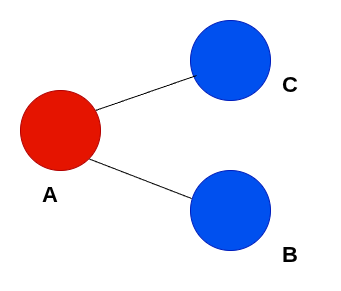
\includegraphics[width=.3\linewidth]{pictures/node_volume_1}
	\caption{Vertex $A$ has an outgoing communication volume of 1 but an edge-cut of 2. Each color represents a partition.}
	\label{fig:edge_vs_volume}
\end{figure}

The performance of a parallel application is generally limited by its slowest processor. This means that even if the computational work is balanced, the communication effort may not be~\cite{buluc_recent_2016}. In such cases, it is more meaningful to minimize the maximum communication load incurred on a single processor rather than the total load across all processors. Neither the standard edge-cut metric nor the total communication volume captures this type of objective.

Furthermore, on many architectures the time to send data, or messages, depends not on geographic distance but on the number of network switches the data must traverse. Although modern machines employ cut-through or wormhole routing to move individual messages quickly between distant processors, the communication network handles many messages simultaneously, and a message between distant processors occupies links that are unavailable to other traffic. Minimizing edge-cut does not account for this locality of communication, and a partition that places frequently communicating processors far apart in the network topology can lead to significant message contention~\cite{hendrickson_graph_2000, buluc_recent_2016}.

%Finally, the time to send a message on a parallel computer depends on both the latency (startup cost) and the message size. GP approaches typically aim to minimize the total communication volume but not the total number of messages sent. Depending on the machine architecture and problem size, message latencies can dominate message volume, making the number of distinct messages a relevant cost factor as well~\cite{hendrickson_graph_2000, buluc_recent_2016}. A few big messages might be more efficient than many small ones. 

%The choice of objective function becomes particulary consequential in the context of parallel computing which is discussed in detail in Section~\ref{}.
%Regardless of the objective function chosen, GP remains a fundamental tool across a wide range of domains. The following section discusses some of its most prominent application areas.
Regardless of the objective function chosen, GP remains a fundamental tool across a wide range of domains. The following sections discuss some of the most used GP algorithms and some of their application areas.

\section{Graph partitioning algorithms} \label{graph_partitioning_algorithms}
In this section we will present some of the most popular GP algorithms used today. The goal is to show some of the differences in the approaches and to highlight their typical use cases. This will help the reader to understand why the multilevel partitioning approach is deemed the best option for large scale graphs. These are, however, only \textit{some} of the existing GP algorithms; a more complete list can be found in~\cite{buluc_recent_2016, 10.1145/3571808}. 

\subsection{Recursive bisection} \label{recursive_bisection}
A popular partitioning method is recursive bisection (RB). Instead of partitioning a graph directly into $k$ subsets, RB first bisects the graph into two roughly equal parts using algorithms such as~\cite{barnard_spectral_bisection, fiduccia_fm, Kernighan_kl}, and then recursively bisects each part until $k$ partitions have been formed. When $k$ is not a power of two, modified schemes are used~\cite{simon_recursive_bisection, chan_spectralkway, KarypisGeorge1998AFaH, hendrickson_multilevel_1995}. Although simple and widely used, RB has been shown to produce suboptimal $k$-way partitions~\cite{simon_recursive_bisection}, since each bisection is made independently without knowledge of the cuts that will follow at deeper levels of the recursion. 

\subsection{Spectral bisection}
Spectral bisection was one of the first methods used to split a graph into two partitions and is still used today~\cite{buluc_recent_2016}. Its approach is to use the eigenvector, also known as the \textit{Fiedler vector}, of the second smallest eigenvalue of the Laplacian matrix to deduce global information of the connectivity of the graph~\cite{fiedler_eigenvector}. In order to form the two partitions, the median value $\overline{m}$ of the Fiedler vector is calculated, and every vertex with a value smaller or equal to $\overline{m}$ is assigned to one partition, and the rest to the other one.

The main computational cost of the spectral method lies in the calculation of the Fiedler vector. To optimize this, Barnard and Simon~\cite{barnard_spectral_bisection} have used a multilevel method to produce an approximation of the Fiedler vector. The spectral method has also been extended to produce a partition for more than only two partitions and to support edge and vertex weights~\cite{hendrickson_multilevel_1995}.

\subsection{Graph growing partitioning} \label{graph_growing}
Another bisection approach is called graph growing partitioning (GGP)~\cite{KarypisGeorge1998AFaH}. GGP is mainly based on breadth-first search (BFS). The core idea is to start from a random vertex and to use BFS to construct a partition. BFS is run until half the vertices are assigned to one partition, the remaining vertices are then assigned to the other one. The choice of starting vertex significantly affects the result, meaning that this algorithm tends to require multiple restarts to obtain a good solution. The GGP approach has also been extended to produce more than two partitions, called \textit{Bubble framework}~\cite{DIEKMANN20001555}. In this version $k$ starting vertices are chosen, evenly distributed in the graph. Starting from these vertices, \textit{k} BFS traversals are performed. Throughout, \textit{Bubble} uses local search algorithms to balance the partitions in the graph. At the end of an iteration, a new starting vertex is chosen for all partitions. The new starting vertex is the vertex with the minimum total distance to all other vertices in the same partition. The algorithm is repeated until no new changes occur in the choice of starting vertices, or no improvement for the partitions is found. The major drawback of this approach is its high computational cost.

\subsection{Streaming graph partitioning}
Streaming data models, where input is processed on the fly rather than all at once, have gained popularity due to their small memory requirements. In the field of GP, the input graph is also passed as a stream, requiring much less space than the graph size~\cite{buluc_recent_2016}. Streaming graph partitioning (SGP) is also very fast, even faster than multilevel algorithms (see Section~\ref{multilevel_gp}). However, these algorithms produce lower quality partitions compared to multilevel approaches. They are nonetheless useful in applications where speed is important, and an initial partition can be obtained from a stronger GP algorithm. For more details about SGP, we refer the reader to~\cite{stanton_streaming_gpp, tsourakakis_fennel, nishimura_streaming_gp}.

\subsection{Multilevel graph partitioning}\label{multilevel_gp}
Multilevel GP is considered to be the most successful heuristic for partitioning large graphs~\cite{buluc_recent_2016, KarypisGeorge1998AFaH, karypis_parallel_1999}. Because of this, multilevel GP was chosen as the base on which to build our new objective function NVOL. In short, the idea is that a graph is coarsened to a smaller graph. Once the graph is at its smallest, an initial partition is performed, and then it is iteratively uncoarsened to the original size. During the uncoarsening, heuristics are applied to improve the partitions. The intuition behind multilevel GP is that it is easy to run intensive partitioning algorithms on the small graph without affecting the total runtime. Additionally, starting from an already good solution, the refinement stage is not costly to perform and can quickly improve the partitions. Chapter~\ref{chap:multilevel-kway} will explain in detail the algorithm, providing the necessary background for understanding how NVOL is integrated into the framework.

\section{Applications of graph partitioning}\label{applications_of_gpp}
Graph partitioning arises in a broad variety of domains. This section highlights several of the most prominent application areas, though the list is by no means exhaustive.

\subsection{Parallel processing}
Perhaps the most widespread application of GP is distributing computational work across the processors of a parallel machine~\cite{langguth_load-balanced_2020}. GP is the standard approach in scientific computing applications such as sparse direct and iterative solvers. When the problem domain remains fixed throughout the computation, the partitioning can be performed once at the outset; this is known as static partitioning~\cite{buluc_recent_2016}. Other common applications in parallel processing include eigenvalue computations~\cite{boman_scalable_2013}, breadth-first search~\cite{buluc_graph_2013}, and algorithms for PageRank and connected components~\cite{salihoglu_gps_2013}. 

\subsection{Complex networks}
GP is also relatively popular in the field of complex networks~\cite{buluc_recent_2016}. Complex networks, in this context, refer to weighted graphs with nontrivial structure arising from real world or modelling processes~\cite{newman_networks_2010}. The objective functions applied in this field are usually domain specific, making it hard to develop optimization algorithms. 

Several application domains illustrate this breadth. In power grids, disturbances and cascading failures may lead to blackouts. GP can be used to isolate self-sufficient islands to prevent propagation of an outage~\cite{li_strategic_2005}. Cut based objective functions are sometimes extended to enhance the robustness of the system~\cite{li_power_2009}.

Geographically embedded networks have experienced a growth in requirements with the advances in
location-aware devices (such as GPS). It is now vital that algorithms be able to analyze networks like these extremely fast. In these networks the vertices commonly represent entities in the real world tied to geographic places. The cut-based approach therefore needs to be reinforced with spatial contiguity constraints~\cite{li_power_2009, buluc_recent_2016}.

Many biological systems can be modeled as graphs~\cite{buluc_recent_2016}, protein-protein interaction or gene co-expression graphs, for example. Partitioning serves multiple purposes ranging from data reduction to the detection of biological processes. More about this field can be found in~\cite{noauthor_wiley_2008}. 

In social networks, community detection is one of the most popular topics. In contrast to traditional GPP, the number of subgroups or partitions is not known a priori~\cite{buluc_recent_2016}. Apart from this, GP has contributed greatly to the development of community detection algorithms~\cite{fortunato_community_2010, newman_community_2013}.

\subsection{VLSI physical design}
VLSI circuit design has historically been one of the primary application areas for graph partitioning~\cite{buluc_recent_2016}. The objective is to decompose a circuit into smaller subcircuits, ranging from gate arrays to complete integrated circuits, while minimizing the total interconnection cost, typically measured as the weight of connections crossing partition boundaries. In this formulation, nodes represent cells (i.e., basic logic or functional units such as gates) and edges represent wires. Scalability is essential, as circuits can contain millions of modules and partitioning constitutes a bottleneck in the overall design flow. Beyond the basic cut objective function, practical VLSI partitioning must also respect domain specific constraints such as I/O placement, groups of cells that are required to remain in the same block, and upper bounds on the cut size between block pairs. Further details can be found in~\cite{kahng_vlsi_2011, cong_multilevel_2003}.

\subsection{Neural networks}
Graph neural networks (GNNs) extend deep learning to graph structured data, enabling the processing of irregular domains that traditional neural network architectures cannot readily handle. However, as graph sizes grow, training GNNs becomes increasingly expensive due to rising communication overhead, particularly in distributed or multi-device settings. Graph partitioning offers a natural approach to this scalability challenge by distributing subgraphs across devices while minimizing inter-device communication.

A recent example is CaPGNN~\cite{song_capgnn_2026}, a parallel full batch GNN training framework designed for multi-GPU servers. CaPGNN combines resource aware graph partitioning with an adaptive caching mechanism that exploits both CPU and GPU memory to reduce redundant data transfers. By taking into account the heterogeneous computational and communication capacities of individual GPUs, the framework achieves substantial reductions in training time with minimal impact on model accuracy. While this is only one instance of a broader trend, it illustrates how classical graph partitioning techniques are finding renewed relevance in the context of modern machine learning workloads.

Another recent example is ParDNN~\cite{qararyah_computational-graph_2021}, an automatic, generic, and non-intrusive partitioning strategy for deep neural networks represented as graphs. Like CaPGNN, this strategy has the goal of minimizing the training time of the model without affecting accuracy. Through their experiments, Qararyah et al. how significant improvements over related work in efficiency, batch size scaling, and training throughput.


	\chapter{Multilevel K-Way Graph Partitioning}\label{chap:multilevel-kway}
This chapter presents the Multilevel K-way Graph Partitioning algorithm which is one of the most widespread GP algorithms. Each section will explain in detail the phases of the multilevel approach with special focus on the techniques used in the partitioner used in this thesis.  

\section{Preliminaries}
The overall structure of a multilevel k-way graph partitioning algorithm is fairly straightforward. The process begins by coarsening the input graph until it is reduced to a size of only a few thousand vertices. At this coarsest level, an initial k-way partitioning is computed using
graph growing algorithm (see Section~\ref{graph_growing})~\cite{KarypisGeorge1998AFaH}. The graph is then uncoarsened back to its original size in successive steps. At each level of uncoarsening, the partitioning is refined to improve quality by exploiting the increased degrees of freedom available at the finer level. Karypis and Kumar demonstrate in~\cite{karypis_multilevelk-way_1998} that this multilevel approach yields high quality partitions, often comparable to, or better than, those produced by recursive bisection~\cite{KarypisGeorge1998AFaH}.

In Figure~\ref{fig:multilevel-overview}, this process is illustrated showing how an initial graph $G_0$ is coarsened until it reaches $G_4$ which is smaller in size. At this level an initial partition is performed on the coarsest graph. After that the graph is step by step projected back to its original size, refining the partition at each level in order to minimize the chosen objective function~\cite{KarypisGeorge1999PMkP}.

The multilevel partitioning problem uses the same definitions as in Section~\ref{sec:gpp}. Additionally, we represent a k-way partition through a vector $P$. The vector has a length of $n$, where $n$ is the number of vertices in the graph. Each element of \textit{P} is an integer between 1 and $k$, indicating the partition the vertex belongs to. Specifically, a vertex $v \in V$ assigned to partition \textit{a} will have $P[v] = a$. The next sections will now explain how each phase works and how the partitions are formed. 

\begin{figure}[h]
	\centering
	\scalebox{0.65}{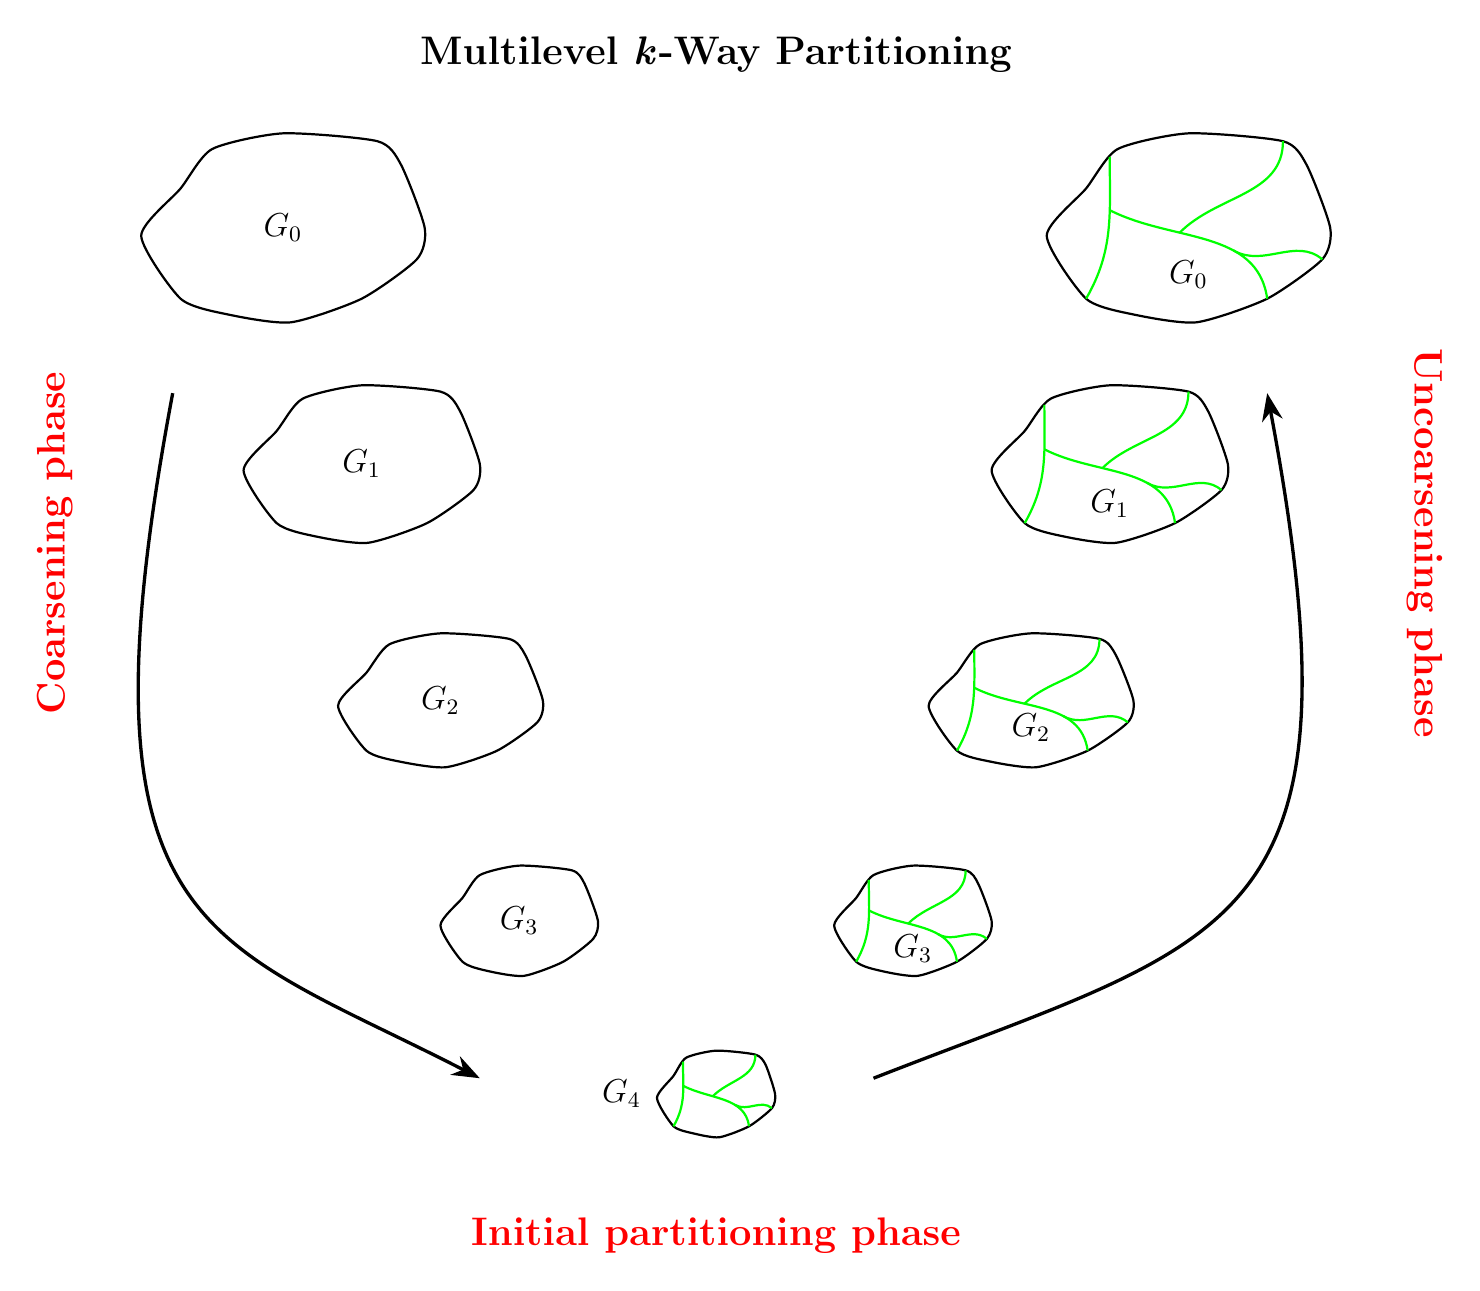
\begin{tikzpicture}[
	graph label/.style={font=\large},
	phase arrow/.style={-{Stealth[length=8pt]}, thick, black},
	phase label/.style={font=\Large\bfseries, text=red},
	pline/.style={green!70!black, thick},
	]
	
	% LEFT SIDE - Coarsening phase
	% G0
	\begin{scope}[shift={(-5, 8)}]
		\draw[thick, fill=white] plot[smooth cycle, tension=0.4] coordinates {
			(1.8, 0)    (1.5, 0.8)   (1.2, 1.1)   (0.0, 1.2)
			(-0.9, 1.0) (-1.3, 0.5)  (-1.8, -0.1) (-1.3, -0.9)
			(-0.7, -1.1) (0.1, -1.2) (1.0, -0.9)  (1.7, -0.4)
		};
		\node[graph label] at (0,0) {$G_0$};
	\end{scope}
	
	% G1
	\begin{scope}[shift={(-4, 5)}]
		\draw[thick, fill=white] plot[smooth cycle, tension=0.4] coordinates {
			(1.5, 0)    (1.25, 0.67)  (1.0, 0.92)   (0.0, 1.0)
			(-0.75, 0.83) (-1.08, 0.42) (-1.5, -0.08) (-1.08, -0.75)
			(-0.58, -0.92) (0.08, -1.0) (0.83, -0.75)  (1.42, -0.33)
		};
		\node[graph label] at (0,0) {$G_1$};
	\end{scope}
	
	% G2
	\begin{scope}[shift={(-3, 2)}]
		\draw[thick, fill=white] plot[smooth cycle, tension=0.4] coordinates {
			(1.3, 0)     (1.08, 0.57)  (0.87, 0.78)   (0.0, 0.85)
			(-0.65, 0.71) (-0.94, 0.35) (-1.3, -0.07) (-0.94, -0.64)
			(-0.51, -0.78) (0.07, -0.85) (0.72, -0.64)  (1.23, -0.28)
		};
		\node[graph label] at (0,0) {$G_2$};
	\end{scope}
	
	% G3
	\begin{scope}[shift={(-2, -0.8)}]
		\draw[thick, fill=white] plot[smooth cycle, tension=0.4] coordinates {
			(1.0, 0)     (0.83, 0.47)  (0.67, 0.64)   (0.0, 0.7)
			(-0.5, 0.58) (-0.72, 0.29) (-1.0, -0.06) (-0.72, -0.52)
			(-0.39, -0.64) (0.06, -0.7) (0.56, -0.52)  (0.94, -0.23)
		};
		\node[graph label] at (0,0) {$G_3$};
	\end{scope}
	
	% G4 with initial partition
	\begin{scope}[shift={(0.5, -3)}]
		\draw[thick, fill=white] plot[smooth cycle, tension=0.4] coordinates {
			(0.75, 0)     (0.63, 0.37)  (0.5, 0.5)    (0.0, 0.55)
			(-0.38, 0.46) (-0.54, 0.23) (-0.75, -0.05) (-0.54, -0.41)
			(-0.29, -0.5) (0.04, -0.55) (0.42, -0.41)  (0.71, -0.18)
		};
		\node[graph label] at (-1.2, -0.0) {$G_4$};
		\draw[green, thick] (-0.42, 0.41) to[out=-90, in=60]
		coordinate[pos=0.35](p1) (-0.54, -0.41);
		\draw[green, thick] (p1) to[out=-27, in=98]
		coordinate[pos=0.35](p2) coordinate[pos=0.65](p3) (0.42, -0.41);
		\draw[green, thick] (p2) to[out=45, in=-90] (0.5, 0.5);
		\draw[green, thick] (p3) to[out=-30, in=140] (0.71, -0.18);
	\end{scope}
	
	% RIGHT SIDE - Uncoarsening phase
	% G3 right
	\begin{scope}[shift={(3, -0.8)}]
		\draw[thick, fill=white] plot[smooth cycle, tension=0.4] coordinates {
			(1.0, 0)     (0.83, 0.47)  (0.67, 0.64)   (0.0, 0.7)
			(-0.5, 0.58) (-0.72, 0.29) (-1.0, -0.06) (-0.72, -0.52)
			(-0.39, -0.64) (0.06, -0.7) (0.56, -0.52)  (0.94, -0.23)
		};
		\node[graph label] at (0,-0.35) {$\small G_3$};
		
		\draw[green, thick] (-0.56, 0.52) to[out=-90, in=60]
		coordinate[pos=0.35](p1) (-0.72, -0.52);
		\draw[green, thick] (p1) to[out=-27, in=98]
		coordinate[pos=0.35](p2) coordinate[pos=0.65](p3) (0.56, -0.52);
		\draw[green, thick] (p2) to[out=45, in=-90] (0.67, 0.64);
		\draw[green, thick] (p3) to[out=-30, in=140] (0.94, -0.23);
	\end{scope}
	
	% G2 right
	\begin{scope}[shift={(4.5, 2)}]
		\draw[thick, fill=white] plot[smooth cycle, tension=0.4] coordinates {
			(1.3, 0)     (1.08, 0.57)  (0.87, 0.78)   (0.0, 0.85)
			(-0.65, 0.71) (-0.94, 0.35) (-1.3, -0.07) (-0.94, -0.64)
			(-0.51, -0.78) (0.07, -0.85) (0.72, -0.64)  (1.23, -0.28)
		};
		\node[graph label] at (0,-0.35) {$G_2$};
		% Wavy horizontals
		\draw[green, thick] (-0.72, 0.64) to[out=-90, in=60]
		coordinate[pos=0.35](p1) (-0.94, -0.64);
		\draw[green, thick] (p1) to[out=-27, in=98]
		coordinate[pos=0.35](p2) coordinate[pos=0.65](p3) (0.72, -0.64);
		\draw[green, thick] (p2) to[out=45, in=-90] (0.87, 0.78);
		\draw[green, thick] (p3) to[out=-30, in=140] (1.23, -0.28);
	\end{scope}
	
	% G1 right
	\begin{scope}[shift={(5.5, 5)}]
		\draw[thick, fill=white] plot[smooth cycle, tension=0.4] coordinates {
			(1.5, 0)    (1.25, 0.67)  (1.0, 0.92)   (0.0, 1.0)
			(-0.75, 0.83) (-1.08, 0.42) (-1.5, -0.08) (-1.08, -0.75)
			(-0.58, -0.92) (0.08, -1.0) (0.83, -0.75)  (1.42, -0.33)
		};
		\node[graph label] at (0,-0.5) {$G_1$};
		% Wavy verticals
		\draw[green, thick] (-0.83, 0.75) to[out=-90, in=60]
		coordinate[pos=0.35](p1) (-1.08, -0.75);
		\draw[green, thick] (p1) to[out=-27, in=98]
		coordinate[pos=0.35](p2) coordinate[pos=0.65](p3) (0.83, -0.75);
		\draw[green, thick] (p2) to[out=45, in=-90] (1.0, 0.92);
		\draw[green, thick] (p3) to[out=-30, in=140] (1.42, -0.33);
	\end{scope}
	
	% G0 right
	\begin{scope}[shift={(6.5, 8)}]
		\draw[thick, fill=white] plot[smooth cycle, tension=0.4] coordinates {
			(1.8, 0)    (1.5, 0.8)   (1.2, 1.1)   (0.0, 1.2)
			(-0.9, 1.0) (-1.3, 0.5)  (-1.8, -0.1) (-1.3, -0.9)
			(-0.7, -1.1) (0.1, -1.2) (1.0, -0.9)  (1.7, -0.4)
		};
		\node[graph label] at (0,-0.6) {$G_0$};
		
		% Partition curves using explicit boundary coordinates
		% 150° ≈ (-1.3, 0.5), 220° ≈ (-1.3, -0.9), 310° ≈ (1.0, -0.9), 60° ≈ (1.2, 1.1)
		
		\draw[green, thick] (-1.0, 0.9) to[out=-90, in=60]
		coordinate[pos=0.35](p1) (-1.3, -0.9);
		
		\draw[green, thick] (p1) to[out=-27, in=98]
		coordinate[pos=0.35](p2) coordinate[pos=0.65](p3)
		(1.0, -0.9);
		
		\draw[green, thick] (p2) to[out=45, in=-90]
		(1.2, 1.1);
		
		\draw[green, thick] (p3) to[out=-30, in=140]
		(1.7, -0.4);
	\end{scope}
	
	% Large curved phase arrows
	\draw[-{Stealth[length=10pt]}, very thick, black]
	(-6.4, 5.9) .. controls (-7.7, -1) and (-6, -1) .. (-2.5, -2.8);
	
	\draw[-{Stealth[length=10pt]}, very thick, black]
	(2.5, -2.8) .. controls (7.1, -1) and (8.8, -1) .. (7.5, 5.9);
	
	% Phase labels
	\node[phase label, rotate=90] at (-7.9, 4) {Coarsening phase};
	\node[phase label] at (0.5, -4.8) {Initial partitioning phase};
	\node[phase label, rotate=-90] at (9.5, 4) {Uncoarsening phase};
	\node[font=\Large\bfseries, text=black!80!black] at (0.5, 10.2) {Multilevel \textit{k}-Way Partitioning};
	
\end{tikzpicture}}
	\caption{The phases of the multilevel k-way partitioning algorithm. During the coarsening phase, the vertices are contracted together and the graph size is successively decreased; during the initial partitioning phase, a k-way partition is performed on the smallest graph; and during the uncoarsening phase, the partitions are successively refined and projected back to a larger graph.}
	\label{fig:multilevel-overview}
\end{figure}

\section{Coarsening Phase}
During the coarsening phase, a sequence of increasingly smaller graphs is constructed maintaining a similar structure to the original graph with fewer degrees of freedom. The most common approach is to aggregate groups of vertices into a single coarse vertex through matching~\cite{buluc_recent_2016, KarypisGeorge1998AFaH}. The coarse vertex has a weight equal to the sum of the weights of all the vertices it contains. Additionally, the coarse vertex receives all the edges of the vertices it contains. Vertices that are not matched are simply copied over to the smaller graph. This process is repeated until we reach a graph $G_m$ with a small enough number of vertices~\cite{karypis_analysis_1995}.

For a given graph $G_i = (V_i, E_i)$, a subset of vertices $V^v_i \subseteq V_i$ is merged into a coarse vertex $v \in V_{i+1}$ for the next coarser graph $G_{i+1}$. The coarse vertex $v$ has weight $w(v) = \sum_{u \in V^v_i}w(u)$. This ensures that the total vertex weight is preserved across coarsening levels. To preserve connectivity, the new vertex $v$ receives the union of the edges of the vertices in $V^v_i$. For any neighbor vertex $u$, the edge weight is $w(\{v,u\}) = \sum_{z\in V^v_i}w(\{z,u\})$. This aggregation strategy preserves structural and weight-related properties of the original graph, thereby enabling efficient and balanced processing at coarser levels~\cite{karypis_multilevelk-way_1998}.
 
As previously mentioned, matching is the most popular coarsening strategy. Formally, the idea is to contract pairs of matched vertices, where we define a matching as a set of edges no two of which share a vertex~\cite{buluc_recent_2016, KarypisGeorge1998AFaH}. Generally, a matching is considered good if it contains many edges. To achieve this, \textit{maximal matchings} are used. A matching is maximal if any edge in the graph, that is not contained in the matching, has at least one of its endpoints matched~\cite{KarypisGeorge1998AFaH}. The following subsection describes in detail the implementation of Sorted Heavy Edge Matching (SHEM), which is the matching algorithm employed by the partitioner used in this thesis. For further reading on other coarsening algorithms, we refer the reader to~\cite{buluc_recent_2016, KarypisGeorge1998AFaH}.

\subsection{Sorted Heavy Edge Matching}
SHEM begins by generating a random permutation of the graph's vertices, which is then sorted based on vertex degrees. Each vertex is gets assigned a bucket by the square of its degree, sorted from lowest to highest. This ordering ensures that low-degree vertices, which have fewer opportunities for matching, are prioritized and thus more likely to be successfully matched. Delaying them would increase the chance of remaining unmatched. Once the vertices are sorted, they are traversed in order. For each unmatched vertex $u$, the algorithm selects the unmatched neighboring vertex $v$ connected to $u$ via the heaviest incident edge. The edge $\{u,v\}$ is then added to the maximal matching $M_i$ and both $u$ and $v$ are marked as matched. If no suitable neighbor exists, the vertex $u$ remains unmatched. This process continues until all vertices have been processed.

The greedy nature of SHEM tends to preserve strong edge connections in the coarser graph, contributing to a significant reduction in total edge weight and, consequently, in the number of edge cuts~\cite{KarypisGeorge1998AFaH, karypis_parallel_1999}. As shown in \cite{karypis_analysis_1995} by Karypis and Kumar, since the coarser graph has smaller edge weight, it also has a smaller edge cut. 

\section{Initial Partitioning Phase}
Once the graph has been coarsened to the smallest level, the initial partitioning is performed. The goal of this stage is to produce $k$ roughly equal partitions before further refinement. Several partitioning algorithms can be used here, including spectral partitioning~\cite{hendrickson_multilevel_1995}, graph growing partitioning~\cite{KarypisGeorge1998AFaH}, and multilevel recursive bisection~\cite{simon_recursive_bisection}, among others. Since the graph is relatively small at this stage, the partitioning is fast. Our partitioner, METIS, uses a multilevel recursive bisection approach. It is also worth mentioning that METIS uses different bisection algorithms based on the graph type. Using the definition in Section~\ref{sec:gpp} we use GGP as the default bisection algorithm.

The a multilevel recursive bisection approach takes the coarse graph and bisects it using GGP. The resulting two subgraphs are then each bisected again. This process is repeated recursively until the desired number of partitions is reached. When the number of partitions is not a power of 2, the algorithm will keep bisecting until one graph has 3 partition remaining. At this level only one of the produced subgraphs will be further bisected. Consider Figure~\ref{fig:tree} where graph $G$ is to be partitioned into 7 groups. At the first level, $G_0$ has 4 partitions remaining while $G_1$ has 3. Since $G_1$ has only 3 partitions remaining, only $G_4$ is bisected further. The left side ($G_0$), on the other hand, continues bisecting until all partitions have been produced.

\begin{figure}[h]
	\centering
	\scalebox{0.65}{
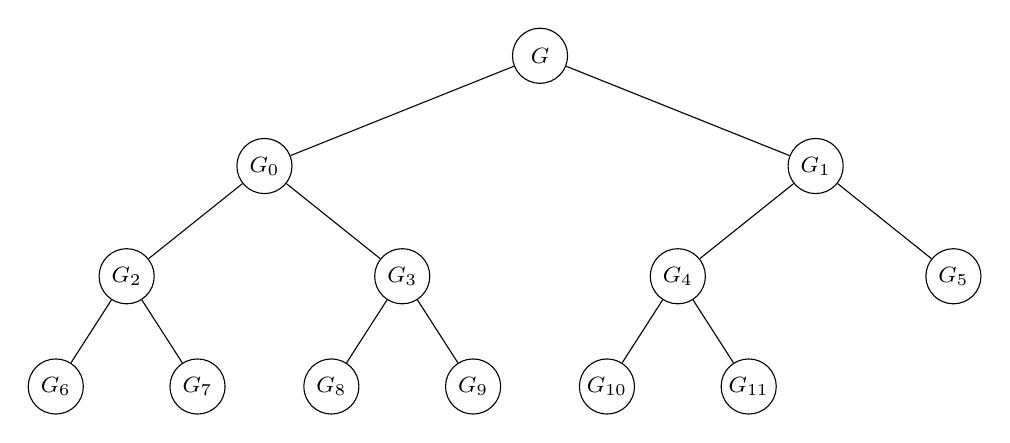
\begin{tikzpicture}[
	level distance=1.4cm,
	every node/.style={circle, draw, minimum size=7mm, inner sep=1pt, font=\footnotesize},
	edge from parent/.style={draw, -},
	level 1/.style={sibling distance=7cm},
	level 2/.style={sibling distance=3.5cm},
	level 3/.style={sibling distance=1.8cm},
	]
	
	\node {$G$}
	child {node {$G_0$}
		child {node {$G_{2}$}
			child {node {$G_6$}}
			child {node {$G_7$}}
		}
		child {node {$G_{3}$}
			child {node {$G_8$}}
			child {node {$G_9$}}
		}
	}
	child {node {$G_1$}
		child {node {$G_{4}$}
			child {node {$G_{10}$}}
			child {node {$G_{11}$}}
		}
		child {node {$G_{5}$}}
	};
	
\end{tikzpicture}
}
	\caption{The process of bisecting a graph into 7 partitions.}
	\label{fig:tree}
\end{figure}

During each bisecting step, GGP is used. As it was described in Section~\ref{graph_growing}, this bisection approach bases itself on BFS. Starting from a random seed it tries to group together vertices connected to each other. At every step it checks that both partitions maintain a weight threshold. Once a partition is computed the graph is further refined using the refinement algorithm proposed by Fiduccia and Mattheyses (FM) in \cite{fiduccia_fm}. The FM refinement algorithm goes through the boundary vertices of the graph, vertices that share at least one edge with a vertex in the other partition. For each step the vertex move that yields the greatest reduction in edge cut (see Section~\ref{subs:objective_functions}) is selected. In order to avoid a subpar solution, FM allows a limited number of moves that worsen the edge cut. This process is repeated over the boundary vertices several times, each time keeping the partition with the lowest edge cut.

It is worth noting that also for our volume based objective we have made use of this approach based on edge cut for the initial partition. There are a few reasons for this. Firstly, the initial partition is going to be heavily refined later during the uncoarsening phase, making the quality of the initial partition not as important. Additionally algorithms like FM are fast and work well with edge cut, optimizing for another objective would make this phase significantly slower. All of these reasons make it reasonable to use edge cut as an objective for this first partitioning.  

\section{Uncoarsening Phase}
The final step is the uncoarsening and refinement phase. During this phase our graph is gradually projected back to the original size. The vertices in a coarse vertex are automatically assigned to the same partition as the coarse vertex. 




%At each level the graph undergoes a refinement of the partitions to ensure better quality with the increased degree of freedom in the finer graph. 



 

%This section will present the multilevel approach as the most important in parallel computing\\
%Coarsening phase\\
%Initial partition \\
%Uncoarsening and refinement\\
%All the way with examples of how Metis is implemented, especially for the volume objective. 	                             	
	\chapter{Communication Volume Calculation} \label{cv_calculation}
This chapter extends the discussion from Section~\ref{sec:greedy_refinement} of Chapter~\ref{chap:multilevel-kway}, where we showed how the change in the objective function's value (the gain) is computed for the edge-cut objective function. Here, we derive the analogous gain computations for two objective functions based on communication volume: the total communication volume objective function (VOL) and our partition-aware communication volume objective function NVOL. The next chapter then shows how these gain calculations are used inside the greedy refinement algorithm.

The chapter is organized into four sections. The first introduces the basic definitions needed to understand communication volume operations. The second describes the gain calculation for VOL, which is more representative of actual communication cost than edge-cut, although it does not necessarily yield a well-balanced result. We treat VOL first because it is the standard approach used by partitioners such as METIS.

The third section presents our novel gain calculation, used by NVOL, which provides finer information about how the volume of each individual partition is affected by a move. Here each vertex has a table representing the partition-specific gain of all possible moves. The section ends with an algorithm that ties the calculation together. The fourth and final section works through a few concrete examples to give the reader a clearer picture of how everything fits together.

\begin{table}[h]
%	\centering
	\label{tab:notation}
	\begin{tabular}{cl}
		\toprule
		\textbf{Symbol} & \textbf{Description} \\
		\midrule
		$G$          & The graph \\
		$V$			& Set of all vertices in the graph\\
		$E$			& Set of all edges in the graph\\
		$V_b$		& Set of all boundary vertices in the graph\\
		$V^{\mathrm{adj}}_i$ & Set of all vertices incident to vertex $i$\\
		$N_i$        & Set of neighboring partitions of vertex $i$ \\
		$N_{iv}$      & Set of partitions neighboring both vertex $i$ and  vertex $v$\\
		$N_{i-v}$    & Set of partitions only neighboring vertex $i$ and not vertex $v$\\
		$w(i)$		& Vertex weight of vertex $i$\\
		$P[i]$		& Partition of vertex $i$\\
		$PV[a]$		& Outgoing communication volume of partition $a$\\
		$C_i[n]$	& Number of edges a vertex $i$ has to a partition $n$\\
		$G_i$		& Gain vector of a vertex $i$\\
		$SG_i$		& Gain table of a vertex $i$\\	
		\bottomrule
	\end{tabular}
	\caption{Notation used in Chapter~\ref{cv_calculation}.}
\end{table}
\section{Basic definitions}
To facilitate understanding of how gain calculation works, we begin by introducing a formal definition of communication volume. Let $G = (V, E)$ be a graph, and let $P$ be the partition vector, where $P[v]$ is the partition a vertex \textit{v} is assigned to. A vertex $u$ is defined as a neighbor of $v$ if there exists an edge $\{u,v\} \in E$. Any vertex adjacent to at least one vertex belonging to a different partition is said to lie on the boundary. We denote the set of all boundary vertices by $V_b \subseteq V$. Formally, $v \in V_b$ if there exists at least one neighbor $u \in V$ such that $\{v,u\} \in E$ and $P[v] \neq P[u]$.

For each boundary vertex $v \in V_b$, let $N_v$ denote the set of distinct partitions (excluding $P[v]$) to which its neighboring vertices belong. The number of partitions contained in $N_v$, defined as $\lvert N_v \rvert$, is the outgoing communication volume of vertex $v$. Note that the number of edges incident to $v$ is not directly relevant for this measure, only the number of distinct neighboring partitions. In Figure~\ref{1}, vertex $A$ has an outgoing communication volume of 2, as it is connected to vertices in two distinct partitions. In contrast, Figure~\ref{2} illustrates a case where vertex $A$ has two edges, both connecting to vertices within the same partition. Consequently, the outgoing communication volume of vertex $A$ is 1, since only a single neighboring partition is involved.

\begin{figure}[H]
	\centering
	\begin{minipage}[b]{.4\textwidth}
		\centering
		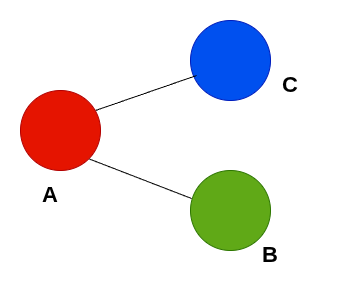
\includegraphics[width=.7\linewidth]{pictures/node_volume_2}
		\caption{Vertex $A$ has an outgoing communication volume of 2. Each color represents a partition.}
		\label{1}
	\end{minipage}\qquad
	\begin{minipage}[b]{.4\textwidth}
		\centering
		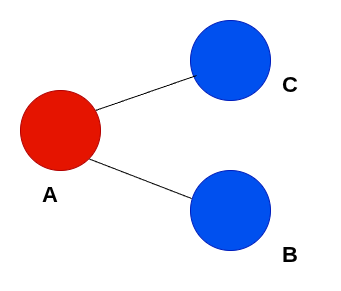
\includegraphics[width=.7\linewidth]{pictures/node_volume_1}
		\caption{Vertex $A$ has an outgoing communication volume of 1. Each color represents a partition.}
		\label{2}
	\end{minipage}
\end{figure}

The total communication volume of the partitioned graph is obtained by summing the outgoing volumes over all boundary vertices:
\begin{equation} \label{total_volume}
	\mathrm{total~volume} = \sum_{v \in V_b} \left| N_v \right|w(v)
\end{equation}
Here, $w(v)$ denotes the weight associated with vertex $v$, which scales its contribution to the outgoing communication volume. Even if the original graph has unit vertex weights, vertices acquire non-unit weights during coarsening as a result of vertex aggregation, and these weights persist during uncoarsening (see Section~\ref{sec:uncoarsening}). In Figure~\ref{tot_vol_example}, all vertices are assumed to have unit weight. The boundary set is $V_b = \{A, B, C, D, E\}$. Note that vertex \textit{F} is not part of this set, as it has no edges connecting to vertices in other partitions.

Applying Equation~\ref{total_volume}, we compute the total communication volume  by summing the contributions of all vertices in the boundary set. Vertices \textit{A}, \textit{C}, and \textit{D} each contribute a volume of 2, while vertices \textit{B} and \textit{E} each contribute a volume of 1. This results in a total communication volume of 8.
\begin{figure}[H]
	\centering
	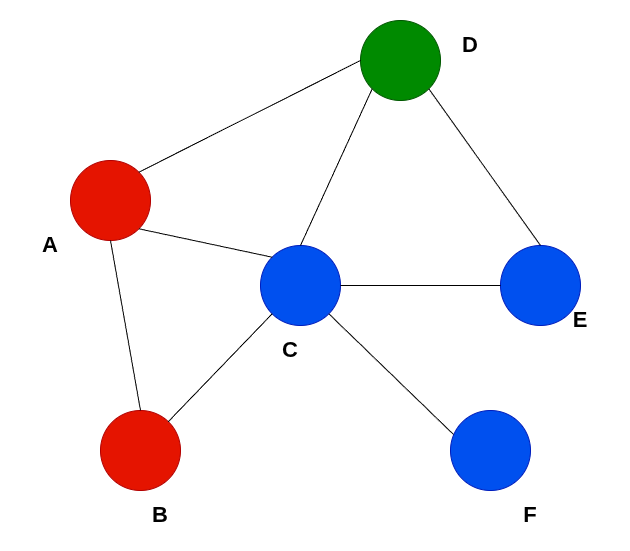
\includegraphics[width=.35\linewidth]{pictures/tot_vol_example}
	\caption{The total communication volume is 8.}
	\label{tot_vol_example}
\end{figure}

\section{VOL gain calculation} \label{METIS gain calculation}
This section describes how the gain resulting from a vertex move is computed for VOL. All definitions are deduced from METIS's implementation, but the approach is standard and applies to any implementation of a total communication volume objective function. The gain for VOL represents the change in total communication volume resulting from relocating a vertex to a new partition: a positive gain indicates a reduction, a negative gain an increase. 

Since communication only arises when an edge connects two vertices belonging to different partitions, a vertex move can only affect the communication volume of its neighboring partitions. For each boundary vertex $i \in V_b$, a partitioner needs to examine all its adjacent vertices $v \in V^{\mathrm{adj}}_i$, where $V^{\mathrm{adj}}_i \subseteq V$ denotes the set of vertices adjacent to $i$. When considering moving a boundary vertex \textit{i}, the gain calculation depends on the relationship that \textit{i} and each of its neighboring vertices have with other partitions. The effect on volume depends on which partitions they share. To support our calculations later, we define, for every vertex \textit{i} and every neighboring vertex \textit{v}
\begin{equation}
	N_{i-v} = N_i \setminus (N_v \cup P[v])
	\quad \text{and} \quad
	N_{iv} = (N_i \cap N_v) \cup P[v]
\end{equation}
representing partitions exclusive to $i$ and partitions shared by $i$ and $v$, respectively. Notice how both sets are subsets of $N_i = N_{i-v} \cup N_{iv}$. Recall that by definition $N_v$ excludes $v$'s own partition $P[v]$. To correctly identify shared partitions, $P[v]$ must therefore be added to $N_{iv}$ and removed from $N_{i-v}$. 

As a concrete example, consider Figure~\ref{tot_vol_example} and suppose the candidate vertex is~$A$, with neighbor~$B$ under consideration. Here, $N_A = \{\mathrm{blue}, \mathrm{green}\}$, while $N_B = \{\mathrm{blue}\}$. Consequently, $N_{A-B} = \{\mathrm{green}\}$, since green is the only partition connected to~$A$ but not to~$B$, whereas $N_{AB} = \{\mathrm{blue}\}$ as both vertices have at least one edge to the blue partition. Keeping \textit{A} as the candidate vertex, consider now neighbor~$C$ with $N_C = \{\mathrm{red}, \mathrm{green}\}$. \textit{A} and \textit{C} have access to the same partitions, meaning that $N_{A-C} = \emptyset$ and $N_{AC} = \{\mathrm{blue}, \mathrm{green}\}$. This example highlights the need for adding $P[C]$ to the sets. The sets would have been $N_{A-C} = \{\mathrm{blue}\}$, $N_{AC} = \{\mathrm{green}\}$ if we had not accounted for $P[C]$. However, from Figure~\ref{tot_vol_example} we can see that the blue partition is shared and not unique to \textit{A}.

Since communication volume is a more complex metric to calculate, and cannot be evaluated on-the-fly like edge-cut, we need to expand our definitions. We define a gain vector $G_i$ with a number of elements equal to the number of partitions, initialized to 0, where $G_i[a]$ represents the total gain obtained by moving vertex $i$ to partition $a$. To determine which contributions to apply to $G_i$, we will also need to count edges between a vertex and a specific partition. Let $C_i[a]$ denote the number of edges connecting $i$ to partition $a$. In Figure~\ref{tot_vol_example}, for example, $C_A[\mathrm{blue}] = 1$, as \textit{A} has only one edge connected to the blue partition, while $C_D[\mathrm{blue}] = 2$, as \textit{D} has two edges connected to the blue partition. 

For a candidate vertex \textit{i} being considered for a move, the gain resulting from moving $i$ to a partition is evaluated by iterating over all neighboring vertices $v \in V^{\mathrm{adj}}_i$. The contribution to $G_i$ depends on the relationship between $i,v$, and their partitions. There are four cases:
\begin{enumerate}[label=\phantom{1.}]\label{METIS CASES}
	\item \textbf{Case 1.} \hypertarget{METIS_case_1} If $P[v] = P[i]$, then moving $i$ to any partition $k \in N_{i-v}$ creates a shared inter-partition connection for $v$, yielding
	\begin{equation}
		G_i[k] \mathrel{-}= w(i)
	\end{equation}
	\item \textbf{Case 2.}\hypertarget{METIS_case_2} If $P[v] \neq P[i]$ and $C_v[P[i]] = 1$, then moving $i$ to any partition $k \in N_{iv}$ eliminates an inter-partition connection for $v$, yielding 
	\begin{equation}
		G_i[k] \mathrel{+}= w(i)
	\end{equation}
	\item \textbf{Case 3.}\hypertarget{METIS_case_3} If $P[v] \neq P[i]$ and $C_v[P[i]] > 1$, then moving $i$ to any partition $k \in N_{i-v}$ introduces a new inter-partition connection for $v$, yielding 
	\begin{equation}
		G_i[k] \mathrel{-}= w(i)
	\end{equation}
	\item \textbf{Case 4.}\hypertarget{METIS_case_4} If $C_i[P[i]] = 0$, i.e., $i$ has no internal degree, then moving $i$ to any partition $k \in N_i$ yields an additional gain contribution of:
	\begin{equation}
		G_i[k] \mathrel{+}= w(i)
	\end{equation}
\end{enumerate}
For every neighboring vertex $v$, we check each cases for every partition in $N_{iv}$, $N_{i-v}$, or $N_i$, depending on the case; together these cases cover all possible changes in communication volume when moving a candidate vertex $i$. 

In Section~\ref{sec:preparation for refinement} the boundary set is filtered using edge-cut gain. When using VOL, we apply the same filtering with the calculations described in this section. Unlike with edge-cut, there is no general equation that determines whether moving a given vertex will yield a positive gain. Instead, we must visit all neighbors of a vertex to correctly evaluate the gains of possible moves. This requires some changes to the preparation phase before refinement. 

METIS solves this by adding the gain calculation as a final step after preparation. Once the graph has been projected and all underlying structures have been recomputed, a full scan of the graph is performed to evaluate the possible gains for every vertex. Algorithm~\ref{alg:cap} presents the full procedure for evaluating the gain vectors of the boundary vertices. In order to filter out negative moves, METIS looks at the highest value in each gain vector and adds only the vertices with non-negative gain to the boundary set. Section~\ref{sec:METIS refinement} shows how the resulting gain vector $G_i$ is used during refinement.

\begin{algorithm}[H]
	\caption{VOL gain calculation}\label{alg:cap}
	\begin{algorithmic}
		\State nparts $\gets k$ 							\Comment{Graph with $k$ partitions}
		\ForAll{$i \in V$}									
			\State $G_i \gets \emptyset$					\Comment{Reset gain vector}
			\If{$|N_i|>0$}										\Comment{Only visit vertices with neighboring partitions}
				\ForAll{$v \in V^{\mathrm{adj}}_i$}					\Comment{Visit all adjacent vertices of i}
					\For{$n = 0$ \textbf{to} $\text{nparts} - 1$}
						\If{n $\in N_i$ \textbf{AND} n $\in N_v$}
							\State $N_{iv}$.add(n)					\Comment{Shared partitions between \textit{i} and \textit{v} ($N_{iv}$)}
						\ElsIf{n $\in N_i$ \textbf{AND} n $\notin N_v$}
							\State $N_{i-v}$.add(n)					\Comment{Partitions only \textit{i} is connected to ($N_{i-v}$)}
						\EndIf
					\EndFor
		
					\If{$P[i] = P[v]$}
						\ForAll{$n \in N_{i-v}$}
							\State $G_i[n] \mathrel{-}= w(i)$				\Comment{Case 1}
						\EndFor
					\ElsIf{$P[i] \neq P[v]$ \textbf{AND} $C_v[P[i]] = 1$}	
						\ForAll{$n \in N_{iv}$}
							\State $G_i[n] \mathrel{+}= w(i)$				\Comment{Case 2}
						\EndFor
					\ElsIf{$P[i] \neq P[v]$ \textbf{AND} $C_v[P[i]] > 1$}
						\ForAll{$n \in N_{i-v}$}
							\State $G_i[n] \mathrel{-}= w(i)$				\Comment{Case 3}
						\EndFor
					\EndIf
				\EndFor	
				\If{$C_i[P[i]] = 0$}
					\ForAll{$n \in N_i$}
						\State $G_i[n] \mathrel{+}= w(i)$				\Comment{Case 4}
					\EndFor
				\EndIf
				\If{MAX($G_i$) $\geq 0$}
					\State BoundarySet.add($i$)			\Comment{Store boundary vertices with positive max gain}
				\EndIf
			\EndIf
		\EndFor	
	\end{algorithmic}
\end{algorithm}

\section{NVOL gain calculation} \label{Partition specific gain calculation}
We now present our novel gain calculation used in NVOL. Whereas VOL aims to minimize the total communication volume of a partitioned graph, NVOL requires finer information to determine what counts as a positive gain for each partition. This is vital for NVOL's refinement, which depends on how each partition's outgoing volume changes. This section shows how to calculate the partition-specific communication volume gain and how to implement it in the multilevel $k$-way partitioning algorithm.

Before diving into the gain calculation, we need to define how the outgoing communication volume is computed for a specific partition. For a partition $a$, the partition-specific outgoing communication volume $PV$ is given by
\begin{equation} \label{partition_volume}
	PV[a] = \sum_{v \in V_b \mid P[v] = a} \left| N_v \right| w(v)
\end{equation}
Consider Figure~\ref{tot_vol_example} again. By using Equation~\ref{partition_volume}, we can calculate the outgoing communication volume of each partition. As before, we assume unit weights. Both vertices in the red partition satisfy $v \in V_b$, as both have edges to other partitions. Vertex $A$ has two neighbor partitions, while $B$ has only one, resulting in $PV[\mathrm{red}] = 3$. The blue partition has only two boundary vertices: $E$ and $C$. Just like the red partition, $PV[\mathrm{blue}] = 3$: $C$ has two neighbors and $E$ has one. Finally, the green partition's only vertex has two neighbors, resulting in $PV[\mathrm{green}] = 2$.

Whereas VOL uses a 1D gain vector $G_i$ that summarizes the total effect of moving $i$ to each destination, NVOL needs to know which partitions absorb that change. We therefore replace the gain vector with a 2D structure that decomposes the gain by affected partition. We introduce the gain table $SG_i$, where each row corresponds to an affected partition and each column to a destination partition for a vertex $i$. The entry $SG_i[a][b]$ represents the gain in outgoing communication volume for partition $a$ when $i$ is moved to partition $b$. This structure, in contrast to the gain vector $G$, is essential for performing partition-specific volume operations. In a graph with $m$ partitions, for a move of vertex $i$ to partition $b$, the total gain satisfies:
\begin{equation}
	\sum_{t=0}^{m-1} SG_i[t][b] = G_i[b]
\end{equation}
i.e., the sum of each column in $SG_i$ equals the corresponding entry in $G_i$. 

With this structure in place, we now describe how its entries are computed. For a candidate vertex \textit{i} being considered for a move, the partition-specific gain resulting from moving $i$ to a partition is evaluated by iterating over all neighboring vertices $v \in V^{\mathrm{adj}}_i$. The contribution to $SG_i$ depends on the relationship between $i,v$, and their partitions. Since this calculation is based on the same communication volume formulation as in Section~\ref{METIS gain calculation}, all volume changes are covered by the same four cases, but the operations performed in each case differ:

\begin{enumerate} [label=\phantom{1.}]
	\item \textbf{Case 1.} \hypertarget{NVOL_case_1} If $P[v] = P[i]$, then moving $i$ to any partition $k \in N_{i-v}$ creates a shared inter-partition connection. This affects the source partition:
	\begin{equation}
		SG_i[P[i]][k] \mathrel{-}= w(i)
	\end{equation}
	\item \textbf{Case 2.} \hypertarget{NVOL_case_2} If $P[v] \neq P[i]$ and $C_v[P[i]] = 1$, then moving $i$ to any partition $k \in N_{iv}$ eliminates an inter-partition connection. This contributes to partition $P[v]$:
	\begin{equation} \label{case 2 nvol}
		SG_i[P[v]][k] \mathrel{+}= w(i)
	\end{equation}	
	\item \textbf{Case 3.} \hypertarget{NVOL_case_3} If $P[v] \neq P[i]$ and $C_v[P[i]] > 1$, then moving $i$ to any partition $k \in N_{i-v}$ introduces a new inter-partition connection. This contributes negatively to partition $P[v]$:
	\begin{equation}
		SG_i[P[v]][k] \mathrel{-}= w(i)
	\end{equation}	
	\item \textbf{Case 4.} \hypertarget{NVOL_case_4} If $C_i[P[i]] = 0$, then moving $i$ to any partition $k \in N_i$ yields an additional gain contribution for the destination partition:
	\begin{equation}
		SG_i[k][k] \mathrel{+}= w(i)
	\end{equation}
\end{enumerate}

The cases above capture the per-neighbor effect of a move. They do not, however, account for the redistribution of $i$'s own contribution to outgoing volume. Moving $i$ removes outgoing volume from the source partition's volume and adds it to the destination's partition. This contribution depends solely on vertex $i$, not on any specific neighbor, so it is applied once per potential move:
\begin{align}
	SG_i[P[i]][k] &\label{eq:source_global_gain} \mathrel{+}= \left| N_i \right| \cdot w(i),\\
	SG_i[k][k]    &\label{eq:destination_global_gain}\mathrel{-}= \left| N_i \right| \cdot w(i).
\end{align}
This is referred to as a global term operation, as it reflects the overall redistribution of communication volume between the source and destination partitions of vertex $i$, rather than interactions with individual neighbor vertices. Equation~\ref{eq:source_global_gain} represents the volume leaving the source partition, while Equation~\ref{eq:destination_global_gain} represents the volume the destination receives. Consequently, it is computed once per vertex move, in contrast to the neighbor-specific gain contributions described earlier, which are evaluated separately for each adjacent vertex. 

Beyond the addition of the global term, both strategies follow the same case structure; the principal difference lies in how they store the gain information. Rather than recording only the magnitude of the change, NVOL also tracks which partition is affected. Section~\ref{sec:NVOL refinement} shows that the gain table is essential for enforcing the logic used in NVOL, which permits moves that improve a single partition regardless of the total communication volume.

Ideally, this calculation should be used to filter the boundary set during the preparation phase. However, due to some implementation constraints discussed in Section~\ref{sec: implementing NVOL}, this was not the case for NVOL. In short, the reason is that storing a gain table for each vertex would require too much memory for it to be a viable option. Instead, the gain calculation is performed during refinement, building the gain table for one boundary vertex at a time. Vertices in the boundary set are filtered using VOL's gain calculation; this is a conservative filter that may exclude some vertices NVOL would otherwise keep. Algorithm~\ref{alg:nvol} shows how the gain table is calculated for a boundary vertex $i$ under consideration.
\vfill
\clearpage
\begin{algorithm}[H]
	\caption{NVOL gain calculation}\label{alg:nvol}
	\begin{algorithmic}
		\State \textbf{Input:} boundary vertex $i$ under consideration
		\State $SG_i[a][b] \gets 0 \ \forall a, b$			\Comment{Reset gain table}
		\State nparts $\gets k$ 							\Comment{Graph with $k$ partitions}
		\ForAll{$v \in V^{\mathrm{adj}}_i$}					\Comment{Visit all adjacent vertices of i}
			\For{$n = 0$ \textbf{to} $\text{nparts} - 1$}
				\If{n $\in N_i$ \textbf{AND} n $\in N_v$}
					\State $N_{iv}$.add(n)					\Comment{Shared partitions between \textit{i} and \textit{v} ($N_{iv}$)}
				\ElsIf{n $\in N_i$ \textbf{AND} n $\notin N_v$}
					\State $N_{i-v}$.add(n)					\Comment{Partitions only \textit{i} is connected to ($N_{i-v}$)}
				\EndIf
			\EndFor
		
			\If{$P[i] = P[v]$}
				\ForAll{$n \in N_{i-v}$}
					\State $SG_i[P[i]][n] \mathrel{-}= w(i)$				\Comment{Case 1}
				\EndFor
			\ElsIf{$P[i] \neq P[v]$ \textbf{AND} $C_v[P[i]] = 1$}	
				\ForAll{$n \in N_{iv}$}
					\State $SG_i[P[v]][n] \mathrel{+}= w(i)$				\Comment{Case 2}
				\EndFor
			\ElsIf{$P[i] \neq P[v]$ \textbf{AND} $C_v[P[i]] > 1$}
				\ForAll{$n \in N_{i-v}$}
					\State $SG_i[P[v]][n] \mathrel{-}= w(i)$				\Comment{Case 3}
				\EndFor
			\EndIf
			\State $N_{iv}\gets \emptyset$							
			\State $N_{i-v}\gets \emptyset$
		\EndFor	
		
		\ForAll{$n \in N_i$}
			\State $SG_i[P[i]][n] \mathrel{+}= |N_i|\cdot w(i)$		\Comment{Global term operations}
			\State $SG_i[n][n] \mathrel{-}= |N_i|\cdot w(i)$
			\If{$C_i[P[i]] = 0$}
				\State $SG_i[n][n] \mathrel{+}= w(i)$				\Comment{Case 4}
			\EndIf
		\EndFor
		
	\end{algorithmic}
\end{algorithm}


\section{Examples}
To better understand the definitions of communication volume and gain, we present a sequence of illustrative examples. Each example highlights a particular configuration and demonstrates how gain contributions arise under different vertex moves.
\subsection{Two partition example}
Consider the graph in Figure~\ref{3}, consisting of five vertices with unit weights. The graph is partitioned into two subsets: the red partition containing vertices $\{A, B, C\}$, and the blue partition containing vertices $\{D, E\}$. Using Equation~\ref{total_volume}, the total communication volume is $4$.

\begin{figure}[h]
	\centering
	\begin{minipage}[t]{.4\textwidth}
		\centering
		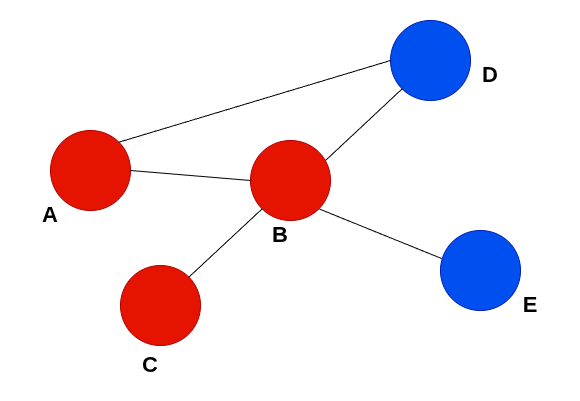
\includegraphics[width=.7\linewidth]{pictures/same_partition_example}
		\caption{Partitioned graph with a volume of 4, each partition has an outgoing volume of 2.}
		\label{3}
	\end{minipage}\qquad
	\begin{minipage}[t]{.4\textwidth}
		\centering
		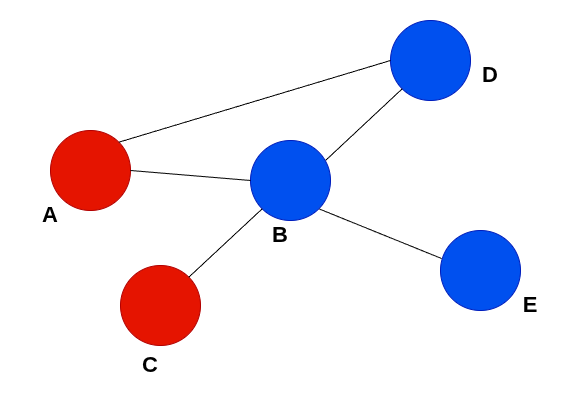
\includegraphics[width=.7\linewidth]{pictures/same_partition_example_moved}
		\caption{Partitinoed graph with a volume of 4, each partition has an outgoing volume of 2 after the move.}
		\label{4}
	\end{minipage}
\end{figure}

Vertex \textit{A} has one edge to the blue partition and contributes $1$ to the communication volume. Vertex \textit{B} has two edges incident to the blue partition, but contributes only $1$ under the given definition. Similarly, vertices \textit{D} and \textit{E} each contribute $1$. In contrast, vertex \textit{C} contributes nothing, as all its incident edges are internal to its partition.
	
Now consider moving vertex \textit{B} from the red partition to the blue partition, as shown in Figure~\ref{4}. We calculate the gain using the global strategy (Section~\ref{METIS gain calculation}). Let \textit{B} be the candidate vertex with neighbors $\{A, C, D, E\}$. Since there are two partitions, the gain vector $G_B$ has size two. In practice, however, $G_B$ effectively has size one, since $G_B[\text{red}]$ is always zero: a vertex moving from its source partition to the source partition is equivalent to no move at all.

\paragraph{Vertex \textit{A}.}
Vertices \textit{A} and \textit{B} are in the same partition and both already have connections to the blue partition. Hence, the set $N_{B-A}$ is empty and no gain contribution arises.

\paragraph{Vertex \textit{C}.}
Vertex \textit{C} lies in the red partition and has no edges to the blue partition. After moving \textit{B}, \textit{C} gains an inter-partition edge, increasing the communication volume. As shown in \hyperlink{METIS_case_1}{Case 1}, this yields a negative gain:
\[
G_B[\text{blue}] \mathrel{-}= 1.
\]
\paragraph{Vertex \textit{D}.}
Vertex \textit{D} is in the blue partition meaning that a move to the blue partition would decrease its volume only if one edge were incident on the red partition. Since \textit{D} has two, \hyperlink{METIS_case_3}{Case 3} does not apply, moving \textit{B} does not change its contribution, hence no case applies.

\paragraph{Vertex \textit{E}.}
Vertex \textit{E} satisfies \hyperlink{METIS_case_2}{Case 2}: it has exactly one connection to the red partition. After the move, this connection disappears, reducing the communication volume and yielding a positive gain:
\[
G_B[\text{blue}] \mathrel{+}= 1.
\]

\hyperlink{METIS_case_4}{Case 4} does not apply, as \textit{B} has multiple connections within its original partition. Summing all contributions yields total gain $0$, so the communication volume remains unchanged.

\paragraph{NVOL gain formulation.}
Using the formulation from Section~\ref{Partition specific gain calculation}, we obtain the same result. We use the table $SG_B$ with size $2\times 1$ (the source column will always be zeroed out just like the source in the gain vector), to store each volume change. As shown above only vertices \textit{C} and \textit{E} contribute:
\[
SG_B[\text{red}][\text{blue}] \mathrel{-}= 1, \quad
SG_B[\text{blue}][\text{blue}] \mathrel{+}= 1.
\]
Additionally, accounting for the direct effect of moving \textit{B} via Equations~\ref{eq:source_global_gain} and~\ref{eq:destination_global_gain}:
\[
SG_B[\text{red}][\text{blue}] \mathrel{+}= 1, \quad
SG_B[\text{blue}][\text{blue}] \mathrel{-}= 1.
\]
The net effect is zero, confirming that neither total nor per-partition volume changes.
\subsection{Three partition example}
We now extend the example to three partitions. Consider the graph in Figure~\ref{three_partition_one_each}, where all vertices have unit weight. The partitions are: red $\{A,B\}$, blue $\{C,D\}$, and green $\{E\}$. The total communication volume is $8$, with partition volumes $3$, $3$, and $2$, respectively.
\begin{figure}[H]
	\centering
	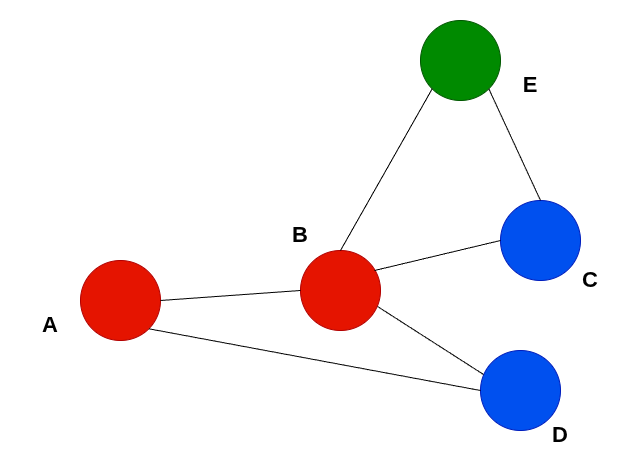
\includegraphics[width=.35\linewidth]{pictures/three_partition_one_each}
	\caption{Partitioned graph with a total communication volume of 8.}
	\label{three_partition_one_each}
\end{figure}
Let \textit{B} be the candidate vertex with neighbors $\{A,C,D,E\}$. Unlike the previous example, \textit{B} may move to either the blue or green partition. Thus, $G_B$ has size 3 and $SG_B$ $3\times 2$.

\paragraph{Vertex \textit{A}.}
Vertex \textit{A} is in the same partition as \textit{B}. Since \textit{A} is connected to the blue partition but not the green partition, \hyperlink{METIS_case_1}{Case 1} applies only for a move to green, introducing a new inter-partition edge:
\[
G_B[\text{green}] \mathrel{-}= 1.
\]

\paragraph{Vertex \textit{C}.}
Vertex \textit{C} is outside the red partition and has exactly one edge to it. By \hyperlink{METIS_case_2}{Case 2}, removing this edge reduces the communication volume. Since \textit{C} is connected to both the blue and green partitions:
\[
G_B[\text{blue}] \mathrel{+}= 1, \quad
G_B[\text{green}] \mathrel{+}= 1.
\]

\paragraph{Vertex \textit{D}.} Vertex \textit{D} has two edges to the red partition. By \hyperlink{METIS_case_3}{Case 3}, a gain change occurs only when the destination partition is not already adjacent to \textit{D}. This holds for the green partition:
\[
G_B[\text{green}] \mathrel{-}= 1.
\]

\paragraph{Vertex \textit{E}.} Vertex \textit{E} is symmetrical to \textit{C}, yielding:
\[
G_B[\text{blue}] \mathrel{+}= 1, \quad
G_B[\text{green}] \mathrel{+}= 1.
\]

Summing contributions gives:
\[
G_B = [0, 2, 0],
\]
indicating that moving \textit{B} to the blue partition reduces the total communication volume by $2$, while moving it to the green partition leaves it unchanged. 

\paragraph{NVOL gain formulation.}
The vector $G_B$ alone does not capture how the volume is redistributed among individual partitions. Using Section~\ref{Partition specific gain calculation}, we compute $SG_B$ as follows.

\paragraph{Vertex \textit{A}.} Vertex \textit{A} follows \hyperlink{NVOL_case_1}{Case 1}for a move to the green partition, yielding:
\[
SG_B[\text{red}][\text{green}] \mathrel{-}= 1
\]

\paragraph{Vertex \textit{C}.} Vertex \textit{C} follows \hyperlink{NVOL_case_2}{Case 2} for both moves, yielding:
\begin{align*}
	SG_B[\text{blue}][\text{blue}] \mathrel{+}= 1 \\
	SG_B[\text{blue}][\text{green}] \mathrel{+}= 1
\end{align*}

\paragraph{Vertex \textit{D}.} Vertex \textit{D} falls under \hyperlink{NVOL_case_3}{Case 3} for the green partition, yielding: 
\[
SG_B[\text{blue}][\text{green}] \mathrel{-}= 1,
\]

\paragraph{Vertex \textit{E}.} Vertex \textit{E} is symmetrical to \textit{C}, yielding:
\begin{align*}
	SG_B[\text{green}][\text{blue}] \mathrel{+}= 1 \\
	SG_B[\text{green}][\text{green}] \mathrel{+}= 1
\end{align*}
Additionally, accounting for the direct effect of moving \textit{B} via Equations~\ref{eq:source_global_gain} and~\ref{eq:destination_global_gain}:
\[
SG_B[\text{red}][\text{blue}] \mathrel{+}= 2, \quad
SG_B[\text{red}][\text{green}] \mathrel{+}= 2,
\]
\[
SG_B[\text{blue}][\text{blue}] \mathrel{-}= 2, \quad
SG_B[\text{green}][\text{green}] \mathrel{-}= 2.
\]
The resulting table $SG_B$ is:
\[
\begin{blockarray}{ccc}
	& \text{blue} & \text{green} \\
	\begin{block}{c(cc)}
		\text{red}   & 2 & 1 \\
		\text{blue}  & -1 & 0 \\
		\text{green} & 1 & -1 \\
	\end{block}
\end{blockarray}
\]

Each column corresponds to a destination partition, and each row describes how a partition's volume changes. One can verify that the column sums recover $G_B$: the sums are 0 (the red partition is implied as no move occurs if the vertex stays in the same partition it already part of), $2+(-1)+1=2$ and $1+0+(-1)=0$ , consistent with $G_B = [0,2,0]$. This formulation provides finer insight: although moving \textit{B} to the green partition leaves the total volume unchanged, it redistributes volume across partitions. In particular, the blue partition experiences an increase in volume at the partition level.

\begin{figure}[H]
	\centering
	\begin{minipage}[t]{.4\textwidth}
		\centering
		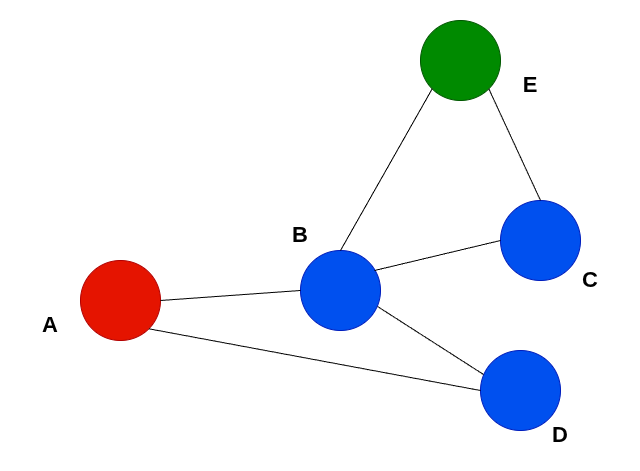
\includegraphics[width=.7\linewidth]{pictures/three_partition_one_each_moved_blue}
		\caption{Partitioned graph has a volume of 6 after \textit{B} is moved to the blue partition}
		\label{three_partition_one_each_moved_blue}
	\end{minipage} \qquad
	\begin{minipage}[t]{.4\textwidth}
		\centering
		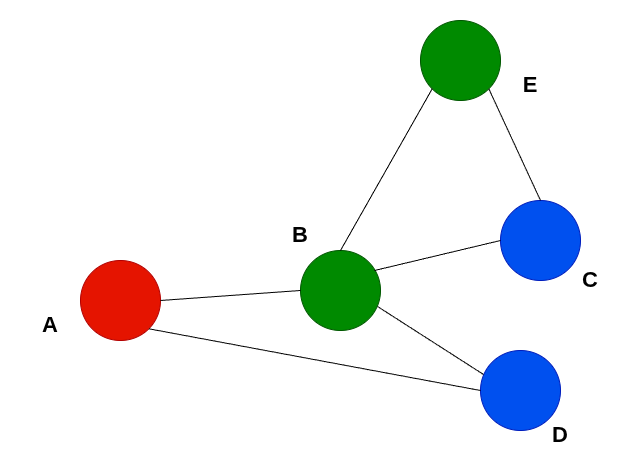
\includegraphics[width=.7\linewidth]{pictures/three_partition_one_each_moved_green}
		\caption{Partitioned graph has a volume of 8 after \textit{B} is moved to the green partition}
		\label{three_partition_one_each_moved_green}
	\end{minipage}
\end{figure}
\subsection{Case 4 example}
None of the preceding examples illustrate a scenario in which Case 4 is relevant. To clarify how such a case may arise and how it affects the communication volume, consider Figure~\ref{case4_example}, where all vertices carry unit weight. The partition assignment is as follows: red $\{A,B,C,G\}$, blue $\{D,E\}$, and green $\{F\}$. The total communication volume is $8$, with individual partition volumes of $3$, $3$, and $2$, respectively. As in the previous example, let $G_C$ have size 3 and $SG_C$  size $3\times 3$.

\begin{figure}[H]
	\centering
	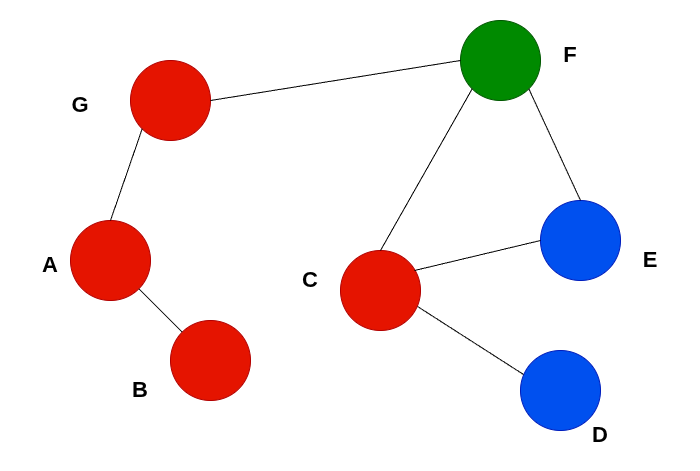
\includegraphics[width=.35\linewidth]{pictures/case4_example}
	\caption{Partitioned graph with a total communication volume of 8.}
	\label{case4_example}
\end{figure}

The candidate vertex is $C$, which has no internal edges within the red partition. Despite the graph containing additional vertices, only the direct neighbors $\{D, E, F\}$ of $C$ need to be visited in order to compute the gain. This illustrates how, even in large graphs, gain computation remains local to the immediate neighborhood of the moving vertex. For conciseness, both computation strategies are consolidated in this example, as they have been thoroughly demonstrated in earlier sections.

\paragraph{Vertex \textit{D}.} Vertex \textit{D} satisfies Case 2 for a move to the blue partition, yielding:
\begin{align*}
	G_C[\text{blue}]\mathrel{+}= 1 \\
	SG_C[\text{blue}][\text{blue}] \mathrel{+}= 1
\end{align*}

\paragraph{Vertex \textit{E}.} Vertex \textit{E} satisfies Case 2 for all possible moves of \textit{C}, yielding: 
\begin{align*}
	G_C[\text{blue}]\mathrel{+}= 1 \\
	G_C[\text{green}]\mathrel{+}= 1 \\
	SG_C[\text{blue}][\text{blue}] \mathrel{+}= 1 \\
	SG_C[\text{blue}][\text{green}] \mathrel{+}= 1
\end{align*}

\paragraph{Vertex \textit{F}.} Vertex $F$ has two edges connecting it to the red partition; however, the set $N_{C-F}$ is empty, meaning Case 3 does not apply and vertex $F$ contributes no change to the gain

\paragraph{Case 4.} Since vertex $C$ has no internal edges, any move will reduce the volume of its source partition. Under normal circumstances, when the candidate vertex has at least one internal edge, moving it leaves the receiving partition's incoming volume unchanged through the candidate. In this case, however, it is necessary to increment the gain for every possible destination partition, yielding:
\begin{align*}
 	G_C[\text{blue}]\mathrel{+}= 1 \\
 	G_C[\text{green}]\mathrel{+}= 1 \\
 	SG_C[\text{blue}][\text{blue}] \mathrel{+}= 1 \\
 	SG_C[\text{green}][\text{green}] \mathrel{+}= 1
\end{align*}
The resulting vector $G_C = [0\,3\,2]$. Accounting for the direct effect of relocating $C$ via Equations~\ref{eq:source_global_gain} and~\ref{eq:destination_global_gain}:
\[
SG_C[\text{red}][\text{blue}] \mathrel{+}= 2, \quad
SG_C[\text{red}][\text{green}] \mathrel{+}= 2,
\]
\[
SG_C[\text{blue}][\text{blue}] \mathrel{-}= 2, \quad
SG_C[\text{green}][\text{green}] \mathrel{-}= 2.
\]
The resulting table $SG_C$ is:
\[
\begin{blockarray}{ccc}
	& \text{blue} & \text{green} \\
	\begin{block}{c(cc)}
		\text{red}   & 2 & 2 \\
		\text{blue}  & 1 & 1 \\
		\text{green} & 0 & -1 \\
	\end{block}
\end{blockarray}
\]
Figures~\ref{case4_example_moved_blue} and~\ref{case4_example_moved_green} show the resulting graphs after moving \textit{C} to the blue and green partitions respectively. The reader can verify that the partition volumes in each case are consistent with the gains predicted by $SG_C$ and $G_C$. Without accounting for Case 4, the gain calculation would be incomplete, potentially leading to incorrect volume estimates when a vertex has no internal edges.
\begin{figure}[H]
	\centering
	\begin{minipage}[t]{.4\textwidth}
			\centering
			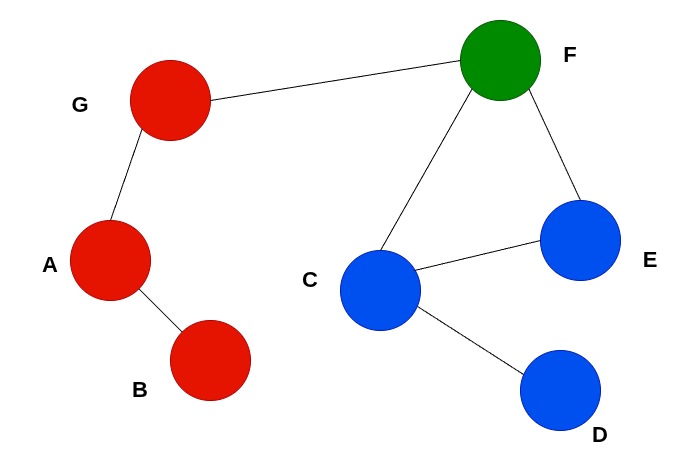
\includegraphics[width=.7\linewidth]{pictures/case4_example_moved_blue}
			\caption{Partitioned graph has a volume of 5 after the move.}
			\label{case4_example_moved_blue}
		\end{minipage}\qquad
	\begin{minipage}[t]{.4\textwidth}
			\centering
			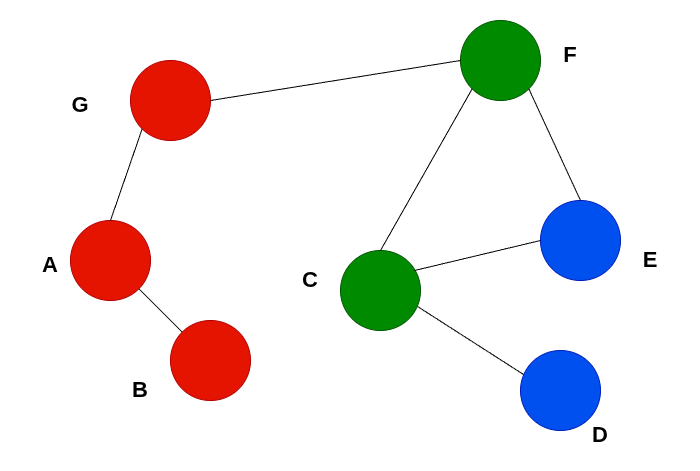
\includegraphics[width=.7\linewidth]{pictures/case4_example_moved_green}
			\caption{Partitioned graph has a volume of 6 after the move.}
			\label{case4_example_moved_green}
		\end{minipage}
\end{figure}

%\section{Implementation}
%%\label{cv_calc_implementation}
%We now describe how the calculation of communication volume change is integrated into the multilevel framework. As mentioned previously, we have used METIS as the base on which to develop NVOL. The following description bridges the formal definitions above and the implemented code.
%
%\subsection{NVOL gain implementation} \label{sec:partition specific gain imp}
	\chapter{Refinement Using Communication Volume} \label{chapter5}
This chapter will discuss how the actual refinement is performed. Using the gains calculated in the previous chapter, we will explain how a vertex move is decided. This chapter will also compare how the choice is made using a total communication volume objective function (VOL) and the partition-aware communication volume used in NVOL.

\section{Refinement using VOL}\label{sec:METIS refinement}
After the preparation phase is completed, refinement starts and the partitioner visits all the vertices in the boundary set. For each vertex $i$, all the neighboring partitions of $i$ are visited, checking the values of the $G_i$ vector. A vertex move is chosen if it improves the total communication volume while maintaining the weight constraints, just like for GR in Section~\ref{sec:greedy_refinement}. The refinement algorithm will look for the move with the highest value in $G_i$ that is allowed by the balance constraints. To prioritize high gain moves, METIS relaxes the balance constraint in proportion to the gain. Using a constant, called the fudge factor $f$, a move to partition $p$ is allowed to exceed the maximum partition weight by $f\cdot G_i[p]$. This allows moves that improve the communication volume significantly at the cost of a few extra vertices in a partition.

When two moves have the same gain, METIS breaks ties using two further criteria: external degree and partition balance. In the case of a tie, it first chooses the move with the highest specific external degree (see Section~\ref{sec:preparation for refinement}). Since all vertices within a coarse vertex are assigned to the same partition upon projection, a move toward a partition with high external degree may reduce volume at finer levels. If instead two candidates have the same gain and the same external degree, the move to the more underweight partition is chosen.

Consider a vertex $i$ being visited in the boundary set during refinement. Algorithm~\ref{alg:ref_vol} shows how METIS chooses vertex moves using the logic described above.
\begin{algorithm}[H]
	\caption{VOL refinement}\label{alg:ref_vol}
	\begin{algorithmic}
		\Require Vertex $i$ with neighbor partitions $N_i[0 \ldots n{-}1]$
		\If{$w(P[i]) - w(i) \geq W^{\min}$}
		\For{$k = n{-}1$ \textbf{downto} $0$}  \Comment{Find first feasible candidate}
		\If{$G_i[N_i[k]] \geq 0$ \textbf{AND}\\
			\hspace*{4.1em}$w(N_i[k]) + w(i) \leq W^{\max} + f \cdot G_i[N_i[k]]$}
		\State \textbf{break}
		\EndIf
		\EndFor
		\If{$k < 0$} \textbf{continue to next vertex} \EndIf
		\For{$j = k{-}1$ \textbf{downto} $0$}  \Comment{Search for a better candidate}
		\State $p_j \gets N_i[j],\; p_k \gets N_i[k]$
		\If{$G_i(p_j) > G_i(p_k)$ \textbf{AND} \\
			\hspace*{4.1em}$w(p_j) + w(i) \leq W^{\max} + f \cdot (G_i(p_j))$}
		\State $k \gets j$ \Comment{Better gain, relaxed balance}
		\ElsIf{$G_i(p_j) = G_i(p_k)$ \textbf{AND}\\
			\hspace*{6.3em}$ED_{p_j}[i] > ED_{p_k}[i]$ \textbf{AND}\\
			\hspace*{6.3em}$w(p_j) + w(i) \leq W^{\max}$}
		\State $k \gets j$ \Comment{Same gain, better connectivity}
		\ElsIf{$G_i(p_j) = G_i(p_k)$ \textbf{AND} \\
			\hspace*{6.3em}$ED_{p_j}[i] = ED_{p_k}[i]$ \textbf{AND} \\
			\hspace*{6.3em}$w(p_j) < w(p_k)$}
		\State $k \gets j$ \Comment{All else equal, prefer underloaded partition}
		\EndIf
		\EndFor
		\State Move $i$ to $N_i[k]$
		\EndIf
	\end{algorithmic}
\end{algorithm}

\section{Refinement using partition-specific communication volume}\label{sec:NVOL refinement}
We now describe how refinement is performed using the partition-specific communication volume objective function in NVOL. In Section~\ref{sec:partition specific gain imp} we explained how, for a boundary vertex $i$, the gain table $SG_i$ is computed. To briefly recall, each entry $SG_i[p][j]$ records the change in outgoing communication volume that partition $p$ would experience if vertex $i$ were moved to neighboring partition $j$. The rows of the table correspond to affected partitions, while the columns correspond to possible destinations. The goal of NVOL is to minimize the maximum outgoing communication volume ($MV^{\mathrm{max}}$) held by any single partition.

\subsection{Move selection}
During refinement, NVOL evaluates every candidate destination for a boundary vertex by inspecting the gain table. For each potential move of vertex $i$ to a destination partition $j$, NVOL determines what the highest volume among all affected partitions would be after the move. If any partition would exceed the current global $MV^{\mathrm{max}}$, the highest volume held by any partition in the entire graph, the move is immediately discarded. As with VOL, NVOL also enforces partition weight constraints: any move must keep the destination partition's weight within the allowed bounds.

NVOL ranks candidate moves according to three criteria, applied in the following order of priority: local $MV^{\mathrm{max}}$, external degree and balance. The first criterion seeks a move that minimizes the local top volume. Out of all the affected partitions, NVOL will choose the move that decreases the top volume of these partitions the most, as long as that top volume is lower than the global $MV^{\mathrm{max}}$. The second criterion is used when two moves have the same local top volume. As a tiebreaker, NVOL favors destinations toward which the considered vertex has a high external degree. This follows the same logic as VOL, aiding moves where the vertex is strongly connected. The final criterion is used when the previous two are tied. NVOL prefers moving vertices to lighter partitions to better balance the weight distribution between the partitions.

\subsection{Encouraging more moves}
A deliberate design choice in NVOL was to promote many vertex moves. Especially when choosing the first candidate, NVOL does not require an immediate improvement of the local top volume. Instead, it chooses any move that leads to a local top that is below the global maximum. This means that in practice NVOL might choose moves that increase the local top volume as long as it is below the global maximum.

The goal with this design is to increase the number of moves NVOL performs during a refinement stage. During testing, we experimented with a stricter criterion that required every accepted move to improve the local top volume. Under this stricter rule, significantly fewer vertices were moved during refinement. On average, the stricter rule performed half as many moves as the more relaxed approach. By encouraging more moves, we encountered two effects. First, NVOL was able to explore more solutions: since more moves were performed, more setups were evaluated. Second, we increased the chance of avoiding getting stuck in a local maximum. If no move could possibly improve the partition's volume, it would remain stuck; by allowing a ``worsening'' move, we increase the chance of finding better solutions. Since the condition still guarantees that the global maximum is never exceeded, the objective's value is protected throughout the process.

To prevent this relaxed condition from accepting moves that are too damaging, NVOL incorporates the fudge factor as a safety mechanism. The fudge factor is used to adjust the maximum allowed partition weight; however, in NVOL we multiply it by the gain for the top partition. Specifically, for a vertex $i$, a partition $m$ with the highest local volume, and a destination partition $j$, we multiply the fudge factor by $SG_i[m][j]$. This ensures that moves that have a negative impact on the local top partition are more likely to be filtered out by the weight constraint. By making the maximum allowed weight smaller, it gets harder to accept a move. In the opposite case, it works as a relaxing factor, allowing moves that positively improve the local top. In this way, $f$ acts as a soft penalty that discourages harmful moves without outright forbidding all non-improving ones. In contrast to VOL, this is used for all criteria other than balance.
\subsection{Implementation of refinement}
For a boundary vertex $i$, NVOL iterates over the neighboring partitions $N_i$. For each candidate destination $j$, it first determines which of the affected partitions would hold the highest volume after the move. In order to do that, it scans all entries $SG_i[k][j]$ for $k \in N_i$ and computes $PV[k] + SG_i[k][j]$, where $PV[k]$ is the volume partition $k$ holds before the move. The partition achieving the highest post-move volume is recorded as the local top partition, with volume tmpVol and partition id tmpPid.

If no candidate has been found yet, NVOL applies the relaxed first condition: destination $j$ is accepted as a candidate if tmpVol does not exceed the global $MV^{\mathrm{max}}$, and the weight constraint $w(j) + w(i) \leq W^{\max} + f \cdot SG_i[\text{tmpPid}][j]$ is satisfied.

Once a first candidate has been found, NVOL tries to find a better destination. A candidate is replaced if the new destination leads to a lower local top volume, using the same weight constraint as above. In the case of a tie, destinations with high external degree $ED_j[i]$ are preferred. If both local top volume and external degree are tied, the destination with the lower current weight is chosen, favoring underloaded partitions. After all neighboring partitions have been considered, vertex $i$ is moved to the final selected destination. The full procedure is given in Algorithm~\ref{alg:ref_nvol}.
\begin{algorithm}[h]
	\caption{NVOL refinement}\label{alg:ref_nvol}
	\begin{algorithmic}
		\Require Vertex $i$ with neighbor partitions $N_i[0 \ldots n{-}1]$; Max partition volume $MV^{\mathrm{max}}$
		\If{$w(P[i]) - w(i) \geq W^{\min}$}
		\State candidateVol $\gets -1 $
		\State destination $\gets -1 $
		\ForAll{$j \in N_i$}
		%		\State $p_j \gets N_i[j]$
		\State tmpVol $\gets 0$
		\State tmpPid $\gets -1$
		%		\State gain $\gets 0$
		\ForAll{$k \in N_i$}
		%			\State $p_k \gets N_i[k]$
			\If{tmpVol$< PV[k] + SG_i[k][j]$}
				\State tmpVol $\gets PV[k] + SG_i[k][j]$
				\State tmpPid $\gets k$
		\EndIf
		%			\State gain $\mathrm{+}= SG_i[p_k][p_j]$
		\EndFor
		\If{candidateVol = -1 \textbf{AND}\\
			\hspace*{4.1em}$MV^{\mathrm{max}} \geq$ tmpVol \textbf{AND} \\
			\hspace*{4.1em}$w(j) + w(i) \leq W^{\max} + f \cdot SG_i[\mathrm{tmpPid}][j]$}
		\State destination $\gets j$ \Comment{Move does not increase max partition volume}
		\State candidateVol $\gets$ tmpVol
		
		\ElsIf{candidateVol != -1 \textbf{AND}\\
			\hspace*{6.3em}candidateVol > tmpVol \textbf{AND}\\
			\hspace*{6.3em}$w(j) + w(i) \leq W^{\max} + f \cdot SG_i[\mathrm{tmpPid}][j]$}
		\State destination $\gets j$ \Comment{Lower local max partition volume after move}
		\State candidateVol $\gets$ tmpVol
		
		\ElsIf{candidateVol != -1 \textbf{AND}\\
			\hspace*{6.3em}candidateVol = tmpVol \textbf{AND}\\
			\hspace*{6.3em}$ED_{j}[i] > ED_{\mathrm{destination}}[i]$ \textbf{AND}\\
			\hspace*{6.3em}$w(j) + w(i) \leq W^{\max} + f \cdot SG_i[\mathrm{tmpPid}][j]$}
		\State destination $\gets j$ \Comment{Same gain, better connectivity}
		\State candidateVol $\gets$ tmpVol
		
		\ElsIf{candidateVol != -1 \textbf{AND}\\
			\hspace*{6.3em} candidateVol = tmpVol \textbf{AND} \\
			\hspace*{6.3em}$ED_{j}[i] = ED_{\mathrm{destination}}[i]$ \textbf{AND} \\
			\hspace*{6.3em}$w(j) < w(\mathrm{destination})$}
		\State destination $\gets j$	\Comment{All else equal, prefer underloaded partition}
		\State candidateVol $\gets$ tmpVol
		\EndIf
		\EndFor
		\State Move $i$ to destination
		\EndIf
	\end{algorithmic}
\end{algorithm}
	\chapter{NVOL tooling support}
This chapter presents some tools used through this thesis that produced the results in Chapter~\ref{chap:results}.

\section{METIS}
For this thesis we used METIS as our multilevel $k$-way partitioner. The METIS framework is open source\footnote{\url{https://github.com/KarypisLab/METIS}}, developed by George Karypis, and widely used. We have also made public a version extended with NVOL\footnote{\url{https://github.com/riccardoie/METIS-with-NVOL}}. Most of the logic behind the multilevel $k$-way algorithm has already been covered in Chapters~\ref{chap:multilevel-kway}--\ref{chapter5}, so we refer the reader to those chapters.

\subsection{Inputs}
METIS requires three inputs: a graph file, the number of partitions, and the objective function. A few optional flags are also available to fine-tune the algorithm.

The graph file must follow a specific structure. The first line is a header whose first two values are the number of vertices and the number of unique edges in the graph. The header may also contain two additional parameters specifying whether the graph has vertex/edge weights and whether it has multiple weights per vertex or edge. Further details can be found in the official manual\footnote{\url{https://github.com/KarypisLab/METIS/blob/master/manual/manual.pdf}}. All graphs used in this work are single-weight, with unit weights on both edges and vertices; note, however, that NVOL also supports graphs with single vertex weights.

The remaining lines of the graph file describe the graph's connectivity: each line corresponds to a vertex, and its entries are the ids of the vertices it is connected to.

\subsection{Output}
Once the algorithm terminates, METIS produces a partition file. This text file contains $n$ lines, where $n$ is the number of vertices in the graph, and each line holds a single integer in the range $[0, k-1]$ indicating the partition the corresponding vertex was assigned to. The partition files are name graphName.part.$k$, where $k$ is the number of partitions. 

\section{Graph Tools}
In this section we will present a few simple tools that were developed during this thesis to display and analyze the results produced by the partitioning algorithm as well as graph formatting. The scripts can all be found in the following repository \footnote{\url{https://github.com/riccardoie/Graph-tools/tree/main}}.

\subsection{calc\_partitions}
To verify and analyze the per-partition outgoing communication volume produced by our experiments, we wrote a simple script, \texttt{calc\_partitions}, that computes it directly from the partition files. It takes two arguments: the original graph filename and the path to the folder containing the partition files. Given these inputs, \texttt{calc\_partitions} computes the outgoing partition volumes for every \texttt{.part.$k$} file associated with that graph. The results are written to a text file divided into sections, one per partition file, each introduced by a header of the form \texttt{graphName.part.$k$}. Within each section, the partitions are listed in order of partition id, from $0$ to $k-1$.

The program works as follows. For every partition file of a graph, it initializes an empty array of length $k$, representing the number of partitions. It then iterates over the graph's vertices, and for each vertex compares its partition with the partition of every neighbor, storing the neighbors' partitions in a set to ensure that each external partition is counted only once per vertex. As shown in Section~\ref{Partition specific gain calculation}, the outgoing communication volume of a partition is the sum of the outgoing communication volumes of the vertices it contains. Once the graph has been fully traversed, the resulting volume array is stored in a dictionary keyed by \texttt{graphName.part.$k$}, and finally written out to the output file.

\subsection{form\_statics}
To collect the per-partition statistics produced by our experiments without recomputing them, we use the script \texttt{form\_statistics}, which processes the files produced by \texttt{calc\_partitions}. For each file, the script reads the contents line by line and parses two types of entries: lines containing \texttt{.part.}, treated as headers marking the beginning of a new partition file's section, and lines starting with \texttt{Pid}, containing the volume of the corresponding partition. The values are grouped by section in a dictionary, and for each group we compute the total outgoing communication volume, the maximum outgoing volume across partitions, the average outgoing volume, and the standard deviation. The results are written to a CSV file, one per input file.

\subsection{graph\_results\_vol}
To evaluate the distribution, we have developed a simple script that plots the partition volumes for a given partition file. The script takes three inputs: the graph file, the number of partitions, and the version identifying the partition file folder. It reads the files output by \texttt{calc\_partitions} and collects all values from the section matching the requested number of partitions. The script is also hardcoded to do the same for the corresponding METIS volumes, and the two sets of volumes are then plotted side by side.

\subsection{stats\_vol}
This script reads the files produced by \texttt{form\_statistics} and plots the results. It takes a graph file name and the version being tested as input, then compares the resulting statistics against the METIS reference values. It produces four plots: the total volume, the maximum partition volume, the percentage difference in maximum partition volume between NVOL and METIS, and the standard deviation of the partition volumes.

%\subsection{model\textunderscore estimates}

\subsection{translate\_to\_metis}
All graphs used in this thesis were in Matrix Market exchange format (.mtx) and therefore needed to be translated into a format METIS could use. The .mtx format is a plain-text format for representing sparse and dense matrices, where each non-zero entry corresponds to an edge in the graph. After the comment lines (prefixed with \%) and a header, each subsequent line lists the two endpoints of an edge: for example, 1 24 denotes an edge between vertex 1 and vertex 24. Our script parses the file and stores each edge as a sorted tuple in a set, which deduplicates entries and discards self-loops. It then builds an adjacency list by iterating over the edge set, appending each vertex to each other's neighbor lists. Since Matrix Market files are 1-indexed while Python lists are 0-indexed, we offset the list indices by one while keeping the vertex ids themselves 1-indexed, as required by the METIS format. Once all edges have been processed, the adjacency list is written as a graph file.
	\chapter{Results}\label{chap:results}

%Explain how things are evaluated
%Look at results
%	max partition vol in different graphs
%	distribution of volume between partitions
%	mpi using Xings model
	\chapter{Conclusions and Future Work} 
This chapter concludes the thesis, evaluating how well the goals we set in the introduction were reached. We look back at the results and evaluate the work done so far. In the final section we look at future work to be done on this project. 


\section{Conclusions}
In Chapter~\ref{chap:introduction} of this thesis we posed two questions: 
\begin{enumerate}
	\item Can a partition-aware objective produce better balanced communication loads than a global one?
	\item Can the performance of a parallel application be improved in practice by using a partition-aware objective?
\end{enumerate}

\subsection{Contributions}
%what was built 
%bullet list of contributions? idk about this one
%set up next subsections
WIP NOT FINISHED

To answer them, we developed NVOL, a novel implementation of a partition-aware objective function based on METIS. Chapters~\ref{cv_calculation} and~\ref{chapter5} describe how the objective function was developed, and Chapter~\ref{chap:NVOL tooling} describes how it was integrated into METIS.

\subsection{Question 1 - Does NVOL improve the volume balance?}
Our results show that NVOL generates partitions with volumes comparable to those produced by METIS when optimizing for total communication volume. NVOL focuses on minimizing the maximum outgoing volume ($W^{\mathrm{max}}$) of any single partition, allowing moves that raise the volume elsewhere as long as the maximum is not increased. This consistently yields partitions with a lower maximum and higher minimum outgoing volume compared to VOL (METIS's total communication volume objective function). The more even distribution is reflected in the lower variance in outgoing volumes, especially in runs with 2 partitions, where NVOL produces perfectly balanced partitions on almost all graphs.

On more regular graphs, NVOL consistently improves on $W^{\mathrm{max}}$. The numerical simulation graphs and the cardiac graphs are particularly notable, with NVOL achieving a lower $W^{\mathrm{max}}$ than VOL in almost every run. On these graphs NVOL also reduces the spread of outgoing volumes across partitions, producing more uniform partition volumes. Notably, on the cardiac graphs and a few others, NVOL even achieves a lower total communication volume than VOL despite not optimizing for that metric.

These results are not universal: NVOL clearly struggles on certain graph structures. Road network graphs in particular proved challenging in our tests, this was the only graph type where NVOL failed to improve on $W^{\mathrm{max}}$ in as many as 45\% of runs. These graphs are sparse, with a few high-degree vertices and many low-degree ones, and this irregular structure prevents NVOL from producing consistent improvements.

The largest graph we managed to test NVOL on was kmer\_U1a, a protein k-mer graph with 67.7 million vertices. This graph is also sparse, with many small, highly connected components. NVOL nevertheless produces a better $W^{\mathrm{max}}$ than VOL and consistently lower standard deviations in the volume values, reaching a reduction in $W^{\mathrm{max}}$ of up to 46.34\%. This suggests that NVOL performs well when given many options, and raises an interesting question: how well would NVOL perform on even larger graphs? On the more negative side, this graph was already too large for NVOL to partition into 2048 parts, making efficiency improvements a priority before scaling further.

This point about NVOL performing better when it has many options is also supported by the results for coPapersDBLP, a graph with a wide variance in edges per vertex. This structure is common in citation networks, which have a few high-degree hub vertices and many low-degree ones. NVOL struggles considerably at low $k$, with the worst result at $-32.09\%$. The trend reverses as $k$ grows, however, peaking at an improvement of $56.70\%$.

We also tested NVOL with imbalance tuning, which produced more variable results. Allowing greater imbalance introduced more instability, with several additional runs failing to improve on $W^{\mathrm{max}}$, though NVOL maintained a positive win rate overall. The main effect of relaxed imbalance appears to be a larger magnitude in both wins and losses. The high variance of these results suggests that imbalance tuning should be treated as a per-run option rather than a default setting.

Taken together, these results answer the first question affirmatively: NVOL produces partitions with more uniform volumes and lower variance compared to METIS's volume objective function. This does push the average partition volume higher, but the increase comes primarily from redistributing the spikes that previously concentrated on a few partitions. NVOL improves the maximum outgoing volume in the partitions, achieving results up to $56.70\%$ compared to METIS's total volume objective.

\subsection{Question 2 - Do the partitions produced by NVOL improve performance?}
The answer to this question is yes, but with an asterisk. NVOL achieves better runtimes than VOL in 65\% of our tests, and maintains a 60\% win rate when imbalance tuning is enabled. On its wins, NVOL improves runtime by an average of 2.61\%, peaking at 6.6\% (without imbalance tuning). 

Some results, such as those for italy\_osm, also show that latency can dominate volume in certain settings. The time spent transmitting the data itself is negligible compared to the latency of initiating each message. As a result, on italy\_osm the tuned NVOL produced a runtime 27.8\% slower than VOL, even though it achieved a 26.61\% lower $W^{\mathrm{max}}$. The slowdown came purely from an increase in the number of partition neighbors: with more partitions to message, the per-message latency dominated the overall runtime.

The coPapersDBLP graph highlights another issue: by producing a higher average volume, NVOL slows down the more heavily loaded processes. Other processes must then wait for them to finish communicating, so the increased per-partition volume affects the overall runtime negatively. This suggests that NVOL will struggle on irregular graphs such as road and citation networks, particularly when they are partitioned into a small number of parts.

These results come with important caveats. We were only able to test on an idealized setup with 32 processors, which significantly limited the number of configurations we could explore. Most of NVOL's greatest improvements appear on partitionings into a large number of parts. Furthermore, these values are only estimates, providing no definitive confirmation that NVOL's runtimes are actually faster on real hardware.

In summary, NVOL does appear to improve efficiency in many cases, but these improvements remain simulated. Future work would require additional testing on real machines to validate these findings. Even so, the estimates we do have are promising and suggest that NVOL's partitions could lead to meaningful performance improvements, especially on graphs partitioned into many parts.

\section{Future Work}\label{chap_future_work}
NVOL shows good potential, delivering consistently strong results across a wide variety of graphs. The conclusions above point out two natural directions for future work: reducing the partitioning time overhead introduced by NVOL, and extending the objective function with hardware-aware information to better target real parallel machines.

\subsection{Improved efficiency} \label{sec:Improved eff}
One of METIS's main strengths is its partitioning speed, and the additional structures and operations introduced by NVOL inevitably affect this, particularly on larger graphs. For small graphs the partitioning time is essentially unchanged, but on larger ones NVOL was observed to be significantly slower than VOL.

The overhead has a straightforward explanation: NVOL adds code to METIS's refinement stage and increases the number of iterations performed there. METIS itself is carefully designed to avoid redundant work, most of the volume operations are performed during graph projection. This way the refinement stage can reuse it rather than reiterating over the graph. NVOL breaks this pattern by recomputing the gain information for each vertex it visits during refinement, effectively repeating work that METIS already performs at projection time.

Three considerations led us not to integrate NVOL's gain calculation directly into the projection stage. First, NVOL has a larger memory requirement than VOL. As described in Chapter~\ref{cv_calculation}, VOL requires a vector whose length equals the number of partitions a vertex neighbors, whereas NVOL requires a table. For a vertex with a gain vector of length $k$, the corresponding gain table has dimensions $(k+1)\times k$, so a gain vector of length 5 already implies a $6 \times 5$ table per vertex. Second, VOL uses incremental updates between moves to keep the volume gains of affected vertices current; implementing the equivalent logic for NVOL was outside the scope of this thesis. Third, and perhaps most decisive, time constraints during development, combined with the considerable effort required to address the first two points, prevented us from pursuing this integration further. 

This decision was nonetheless preceded by an attempt at the integration. Our strategy allocated the exact memory needed for each gain table and deallocated it once the corresponding vertex left the boundary; gain updates were handled by simply recomputing all neighbors of the moved vertex. In principle this is much closer to what VOL does and should have improved performance. In practice, however, the algorithm became even slower than the original NVOL implementation, with the frequent allocation and deallocation of memory as the dominant cost. A better solution would be to allocate a single block of memory at projection time, sized from an estimate of how many boundary vertices the finer graph will contain, with additional logic to extend the block when the estimate falls short and to release it once refinement completes. Combined with proper incremental updates of neighboring vertices' gains after each move, this would allow NVOL to partition in a time frame close to VOL, at the cost of higher memory use.

\subsection{Introduce hardware knowledge}
Using the partition-specific implementation of NVOL, it would be interesting to incorporate some of the logic presented in~\cite{Xing_of_Heterogeneous} to further improve actual runtime. Currently, we partition using communication volume and then model the runtime of each partition based on a set of constants and the incoming volume. With the right adaptations, NVOL could already evaluate this during refinement. Changing NVOL's volume calculations from outgoing to incoming volume is non-trivial, but it has the potential for even larger improvements.

The general idea would be to extend METIS to accept additional parameters describing the latencies and bandwidth of the machine running the partitions. Then, during refinement, one could use the equations shown in Section~\ref{sec:model estimates} to evaluate candidate moves. This would increase the chance of producing a partitioning that performs well on the target parallel machine. NVOL's per-partition structure is essential to such an approach.

This could be extended further to optimize for heterogeneous machines. So far we have only considered tests on machines where each component was identical, but in reality modern parallel computers are larger and more complex. Their heterogeneous structure therefore brings an added level of complexity that can be exploited. In~\cite{Xing_of_Heterogeneous}, the authors also develop models for such setups. With the right structures in place, NVOL could support this logic as well.                   
	\backmatter{}
	\printbibliography
%	\appendix
\end{document}